% Options for packages loaded elsewhere
\PassOptionsToPackage{unicode}{hyperref}
\PassOptionsToPackage{hyphens}{url}
\documentclass[
  11pt,
]{article}
\usepackage{xcolor}
\usepackage[left=3cm,right=3cm,top=2.5cm,bottom=2.5cm]{geometry}
\usepackage{amsmath,amssymb}
\setcounter{secnumdepth}{5}
\usepackage{iftex}
\ifPDFTeX
  \usepackage[T1]{fontenc}
  \usepackage[utf8]{inputenc}
  \usepackage{textcomp} % provide euro and other symbols
\else % if luatex or xetex
  \usepackage{unicode-math} % this also loads fontspec
  \defaultfontfeatures{Scale=MatchLowercase}
  \defaultfontfeatures[\rmfamily]{Ligatures=TeX,Scale=1}
\fi
\usepackage{lmodern}
\ifPDFTeX\else
  % xetex/luatex font selection
\fi
% Use upquote if available, for straight quotes in verbatim environments
\IfFileExists{upquote.sty}{\usepackage{upquote}}{}
\IfFileExists{microtype.sty}{% use microtype if available
  \usepackage[]{microtype}
  \UseMicrotypeSet[protrusion]{basicmath} % disable protrusion for tt fonts
}{}
\usepackage{setspace}
\makeatletter
\@ifundefined{KOMAClassName}{% if non-KOMA class
  \IfFileExists{parskip.sty}{%
    \usepackage{parskip}
  }{% else
    \setlength{\parindent}{0pt}
    \setlength{\parskip}{6pt plus 2pt minus 1pt}}
}{% if KOMA class
  \KOMAoptions{parskip=half}}
\makeatother
\usepackage{longtable,booktabs,array}
\usepackage{caption}
\captionsetup[table]{skip=6pt}
\newcounter{none} % for unnumbered tables
\usepackage{calc} % for calculating minipage widths
% Correct order of tables after \paragraph or \subparagraph
\usepackage{etoolbox}
\makeatletter
\patchcmd\longtable{\par}{\if@noskipsec\mbox{}\fi\par}{}{}
\makeatother
% Allow footnotes in longtable head/foot
\IfFileExists{footnotehyper.sty}{\usepackage{footnotehyper}}{\usepackage{footnote}}
\makesavenoteenv{longtable}
\usepackage{graphicx}
\makeatletter
\newsavebox\pandoc@box
\newcommand*\pandocbounded[1]{% scales image to fit in text height/width
  \sbox\pandoc@box{#1}%
  \Gscale@div\@tempa{\textheight}{\dimexpr\ht\pandoc@box+\dp\pandoc@box\relax}%
  \Gscale@div\@tempb{\linewidth}{\wd\pandoc@box}%
  \ifdim\@tempb\p@<\@tempa\p@\let\@tempa\@tempb\fi% select the smaller of both
  \ifdim\@tempa\p@<\p@\scalebox{\@tempa}{\usebox\pandoc@box}%
  \else\usebox{\pandoc@box}%
  \fi%
}
% Set default figure placement to htbp
\def\fps@figure{htbp}
\makeatother
% definitions for citeproc citations
\NewDocumentCommand\citeproctext{}{}
\NewDocumentCommand\citeproc{mm}{%
  \begingroup\def\citeproctext{#2}\cite{#1}\endgroup}
\makeatletter
 % allow citations to break across lines
 \let\@cite@ofmt\@firstofone
 % avoid brackets around text for \cite:
 \def\@biblabel#1{}
 \def\@cite#1#2{{#1\if@tempswa , #2\fi}}
\makeatother
\newlength{\cslhangindent}
\setlength{\cslhangindent}{1.5em}
\newlength{\csllabelwidth}
\setlength{\csllabelwidth}{3em}
\newenvironment{CSLReferences}[2] % #1 hanging-indent, #2 entry-spacing
 {\begin{list}{}{%
  \setlength{\itemindent}{0pt}
  \setlength{\leftmargin}{0pt}
  \setlength{\parsep}{0pt}
  % turn on hanging indent if param 1 is 1
  \ifodd #1
   \setlength{\leftmargin}{\cslhangindent}
   \setlength{\itemindent}{-1\cslhangindent}
  \fi
  % set entry spacing
  \setlength{\itemsep}{#2\baselineskip}}}
 {\end{list}}
\usepackage{calc}
\newcommand{\CSLBlock}[1]{\hfill\break\parbox[t]{\linewidth}{\strut\ignorespaces#1\strut}}
\newcommand{\CSLLeftMargin}[1]{\parbox[t]{\csllabelwidth}{\strut#1\strut}}
\newcommand{\CSLRightInline}[1]{\parbox[t]{\linewidth - \csllabelwidth}{\strut#1\strut}}
\newcommand{\CSLIndent}[1]{\hspace{\cslhangindent}#1}
\setlength{\emergencystretch}{3em} % prevent overfull lines
\providecommand{\tightlist}{%
  \setlength{\itemsep}{0pt}\setlength{\parskip}{0pt}}
% Paragraph scaffolding for manuscript revision.
%
% Two environments, presented in this order per paragraph:
%
%   rgt   -- author's rewrite (initially a placeholder)
%            small, italic, dark blue
%   orig  -- original Claude-authored draft, and until the rewrite
%            replaces it, the body text of the manuscript
%            normal size, gray
%
% The `bullets' environment (a boiled-down topic sentence plus bullet
% points, one per paragraph) is no longer used inside manuscripts:
% those blocks now live in a companion bullets.Rmd supplement in the
% same report directory, which typesets them as plain \textbf{} +
% itemize and needs no part of this file. The definition is retained
% only so that a stray block left in a document still compiles.
%
% This file is identical across every manuscript that includes it.
% It previously existed in two variants that swapped the sizes of
% rgt and orig, so the same markup rendered differently depending on
% which repository the manuscript lived in. The variant retained here
% keeps orig at full size because orig, not rgt, currently carries
% the prose in every manuscript in the pool.

\usepackage{xcolor}

\newcounter{pgraph}

\newenvironment{bullets}{%
  \stepcounter{pgraph}%
  \begin{quote}\small\sffamily\color[gray]{0.30}%
  {\normalfont\scriptsize\color[gray]{0.58}[\thepgraph]\enspace}}{%
  \end{quote}}

\newenvironment{rgt}{%
  \begin{quote}\small\itshape\color[RGB]{20,60,160}}{%
  \end{quote}}

\newenvironment{orig}{%
  \begin{quote}\normalsize\color[gray]{0.55}}{%
  \end{quote}}

% backward compat alias
\newenvironment{claudecode}{\begin{orig}}{\end{orig}}
%% tools/stamp.tex
%% Provenance footer for PDFs rendered from this project.
%% Vendored by zzcollab; this file is not project-specific. The
%% footer prints the source document and the time of rendering.
%% The git version is defined here too, and so is available to a
%% project that wants it on the page, but it is left off the
%% default footer: it already names the staged copy in share/ and
%% appears in its manifest row. All values are supplied at render
%% time by tools/stamp-render.R, which writes a small generated
%% file that redefines the macros below. The \providecommand
%% defaults keep a bare LaTeX compile working when the document is
%% built without the wrapper.
\usepackage{fancyhdr}
\usepackage{xcolor}
\providecommand{\stampsource}{\detokenize{(source not recorded)}}
\providecommand{\stamptime}{(time not recorded)}
\providecommand{\stampversion}{\detokenize{(version not recorded)}}
\setlength{\footskip}{40pt}
\newcommand{\stampfootcontent}{%
  \footnotesize\color{gray}%
  \parbox[b]{\textwidth}{%
    \stamptime\hfill\thepage\\[2pt]%
    \ttfamily\raggedright\stampsource}}
\pagestyle{fancy}
\fancyhf{}
\fancyfoot[C]{\stampfootcontent}
\renewcommand{\headrulewidth}{0pt}
\renewcommand{\footrulewidth}{0.4pt}
%% The title page uses the `plain` page style; redefine it so the
%% stamp appears there too.
\fancypagestyle{plain}{%
  \fancyhf{}%
  \fancyfoot[C]{\stampfootcontent}%
  \renewcommand{\headrulewidth}{0pt}%
  \renewcommand{\footrulewidth}{0.4pt}}
\renewcommand{\stampsource}{\textasciitilde{}/\allowbreak{}prj/\allowbreak{}res/\allowbreak{}36-pmsimstats-ng/\allowbreak{}pmsimstats-ng/\allowbreak{}analysis/\allowbreak{}report/\allowbreak{}04-treatment-main-effect/\allowbreak{}report.Rmd}
\renewcommand{\stamptime}{2026-08-20 17:18 PDT}
\renewcommand{\stampversion}{\detokenize{faccea3-wip}}
\usepackage{amsmath}
\usepackage{amssymb}
\usepackage{booktabs}
\usepackage{longtable}
\usepackage{float}
\usepackage[mathlines]{lineno}
\linenumbers
\usepackage{booktabs}
\usepackage{longtable}
\usepackage{array}
\usepackage{multirow}
\usepackage{wrapfig}
\usepackage{float}
\usepackage{colortbl}
\usepackage{pdflscape}
\usepackage{tabu}
\usepackage{threeparttable}
\usepackage{threeparttablex}
\usepackage[normalem]{ulem}
\usepackage{makecell}
\usepackage{xcolor}
\usepackage{bookmark}
\IfFileExists{xurl.sty}{\usepackage{xurl}}{} % add URL line breaks if available
\urlstyle{same}
% fallback for those not using the hyperref driver hyperxmp:
\makeatletter
\@ifundefined{xmpquote}{\newcommand{\xmpquote}[1]{#1}}{}
\makeatother
\hypersetup{
  pdftitle={Comparative Statistical Power of N-of-1 Trials versus Randomized Controlled Trials: A Simulation Study of Prazosin for PTSD Nightmares},
  pdfauthor={pmsimstats team},
  hidelinks,
  pdfcreator={LaTeX via pandoc}}

\title{Comparative Statistical Power of N-of-1 Trials versus Randomized Controlled Trials: A Simulation Study of Prazosin for PTSD Nightmares}
\author{pmsimstats team}
\date{August 20, 2026}

\begin{document}
\maketitle
\begin{abstract}
\textbf{Background:} N-of-1 trials offer a promising approach for precision medicine by evaluating treatment effects within individual patients through repeated crossover designs. Their statistical properties relative to traditional randomized controlled trials remain incompletely characterized across clinically realistic effect-size and carryover regimes. \textbf{Methods:} We conducted an ADEMP-compliant Monte Carlo simulation study comparing the statistical power of aggregated N-of-1 hybrid trials versus parallel-group RCTs for detecting treatment effects of prazosin in reducing PTSD nightmares. The N-of-1 design enrolled 35 individuals each completing 8-period crossover trials analyzed by a linear mixed-effects model with continuous-time AR(1) residuals; the RCT arm used ANCOVA at matched sample size \(N = 35\). Carryover-contaminated placebo periods were excluded from the N-of-1 analysis before fitting. We ran \(n_{\text{sim}} = 2{,}000\) replicates per cell, uniform across all primary and sensitivity analyses. \textbf{Results:} The aggregated N-of-1 hybrid dominated the parallel-group RCT across the full effect-size range. At a true effect of \(-2.0\) nightmares per week, N-of-1 power was 1.000 versus 0.675 (Monte Carlo standard error, MCSE, 0.010) for the RCT; at \(-1.0\), N-of-1 power was 0.830 (MCSE 0.008) versus 0.230 (MCSE 0.009). Bias was negligible in both designs. Coverage of nominal-95\% CIs was 0.940--0.949 for the N-of-1 arm and 0.939 for the RCT arm across all effect sizes. \textbf{Conclusions:} Aggregated N-of-1 hybrid trials achieve substantially higher statistical power than parallel-group RCTs at matched sample size when within-subject carryover is managed by period exclusion. The efficiency advantage is largest in the small-to-moderate effect-size regime where parallel-group RCTs are essentially underpowered. \textbf{Keywords:} N-of-1 trials; randomized controlled trials; statistical power; crossover design; carryover effects; PTSD; prazosin; precision medicine.
\end{abstract}

{
\setcounter{tocdepth}{2}
\tableofcontents
}
\setstretch{1.1}
\section{Abstract}\label{abstract}

\begin{claudecode}
**Background.** Aggregated N-of-1 trial designs and parallel-group
randomized controlled trials are the two principal methodological
alternatives for evaluating treatment effects under substantial
individual heterogeneity. The published literature characterizes
the variance-component foundations of each design separately, but
has not, to the best of our knowledge, delivered a comprehensive
sample-size and power comparison across clinically realistic
effect-size and carryover regimes that admits Monte Carlo
standard-error reporting within the ADEMP framework of Morris,
White, and Crowther [-@morris2019simulation].

**Methods.** We conduct an ADEMP-compliant Monte Carlo simulation
study comparing the aggregated N-of-1 hybrid design to a
parallel-group RCT at matched sample size $N = 35$, across a grid
of true-effect sizes $\{0, -0.5, -1.0, -2.0\}$ nightmares per
week, calibrated to the prazosin/PTSD reference application. The
hybrid N-of-1 arm fits an `nlme::lme` model with continuous-time
AR(1) residual correlation; the parallel-group RCT arm fits a
baseline-adjusted linear model (ANCOVA). Carryover-contaminated
placebo periods are excluded before fitting the N-of-1 model.
Each cell is run at $n_{\text{sim}} = 2{,}000$ replicates; null
cells (true effect zero) provide explicit Type I error checks.
Estimands include power, empirical effect-size bias, empirical SE,
model SE, and nominal-95% CI coverage; all performance measures
are reported with Monte Carlo standard errors. Sensitivity sweep
S1 examines carryover half-lives in $\{0.5, 1, 3, 5, 7\}$ days.

**Results.** The aggregated N-of-1 hybrid dominated the
parallel-group RCT across the entire effect-size range. At true
effect $-2.0$, N-of-1 power was $1.000$ versus parallel-group
$0.675 \pm 0.010$; at $-1.0$, $0.830 \pm 0.008$ versus
$0.230 \pm 0.009$; at $-0.5$, $0.311 \pm 0.010$ versus
$0.104 \pm 0.007$. The two power curves did not cross within the
simulated range; gaps exceeded five combined MCSEs at every
non-null effect size. The relative N-of-1-to-RCT power ratio was
approximately $3.0\times$ at the moderate-effect $-0.5$ cell.
Bias was negligible across all cells for both designs. Coverage of
nominal-95% CIs was 0.940--0.949 for the N-of-1 arm and 0.939 for
the RCT arm, each within two MCSEs of the nominal level. The
N-of-1 analysis was insensitive to the true carryover half-life,
confirming robustness of the period-exclusion strategy. Type I
error was $0.051 \pm 0.005$ for the N-of-1 hybrid and
$0.061 \pm 0.005$ for the RCT; the RCT rate is marginally above
nominal, consistent with small-sample effects in $\text{lm}$ at
$N = 35$.

**Conclusions.** Aggregated N-of-1 hybrid trials achieve
substantially higher statistical power than parallel-group RCTs at
matched sample size when individual variability is substantial and
within-subject carryover is manageable. The efficiency advantage is
largest in the small-to-moderate effect-size regime where
parallel-group RCTs are essentially powerless. Trial designers in
precision-medicine settings with high between-patient
variability should consider the aggregated N-of-1 design as the
preferred default.
\end{claudecode}

\section{Introduction}\label{introduction}

\begin{rgt}
Lorem ipsum dolor sit amet, consectetur adipiscing elit, sed do eiusmod tempor incididunt ut labore et dolore magna aliqua.

\end{rgt}

\begin{orig}
Clinical research has moved steadily toward precision-medicine
approaches that recognize substantial between-patient variance in
treatment response\textsuperscript{\citeproc{ref-lillie2011}{1},\citeproc{ref-nam2021expanding}{2}}.
Traditional randomized controlled trials (RCTs), while remaining the
standard for establishing population-level treatment effects, may not
capture the between-patient variability that is central
to precision-medicine therapeutic decision-making\textsuperscript{\citeproc{ref-kravitzSinglepatientNof1Trials2014}{3},\citeproc{ref-marshallScopingReviewRandomized2022}{4}}.

\end{orig}

\begin{rgt}
Lorem ipsum dolor sit amet, consectetur adipiscing elit, sed do eiusmod tempor incididunt ut labore et dolore magna aliqua.

\end{rgt}

\begin{orig}
N-of-1 trials, also known as single-patient crossover trials, evaluate
treatment efficacy within individual patients through repeated crossover
periods\textsuperscript{\citeproc{ref-Miller1999n}{5},\citeproc{ref-vohraCONSORTExtensionReporting2015}{6}}. In these
designs each patient serves as their own control, which reduces the
confounding effect of between-patient variability while providing
individual-level treatment-effect estimates\textsuperscript{\citeproc{ref-zucker2010}{7},\citeproc{ref-schmidBayesianModelsNof12021}{8}}. When
appropriately aggregated across patients, N-of-1 trials can support
population-level inference while simultaneously informing individual
treatment decisions\textsuperscript{\citeproc{ref-chenComparisonAggregatedNof12020}{9},\citeproc{ref-araujoComparisonFourMethods2014}{10}}.

\end{orig}

\subsection{Methodological Considerations in N-of-1 Trial Design}\label{methodological-considerations-in-n-of-1-trial-design}

\begin{rgt}
Lorem ipsum dolor sit amet, consectetur adipiscing elit, sed do eiusmod tempor incididunt ut labore et dolore magna aliqua.

\end{rgt}

\begin{orig}
The statistical analysis of N-of-1 trials presents methodological
challenges that differ substantially from those of traditional
parallel-group designs\textsuperscript{\citeproc{ref-schmidStatisticalDesignAnalytic2014}{11},\citeproc{ref-sennAnalysisContinuousData2024}{12}}. Among the key considerations are
the appropriate handling of carryover effects, period effects, and
temporal trends within individual patients\textsuperscript{\citeproc{ref-tangTtestsNof1Trials2020}{13},\citeproc{ref-yapBehavioralCarryoverEffect2024}{14}}.
Carryover effects, representing the residual influence of treatment
from previous periods, are particularly critical in crossover
designs and can substantially affect both the validity and the
power of statistical analyses\textsuperscript{\citeproc{ref-liuConsiderationsCrossoverDesign2021}{15},\citeproc{ref-patsopoulosUnderstandingControlledTrials2011}{16}}.

\end{orig}

\begin{rgt}
Lorem ipsum dolor sit amet, consectetur adipiscing elit, sed do eiusmod tempor incididunt ut labore et dolore magna aliqua.

\end{rgt}

\begin{orig}
The aggregation of individual N-of-1 trials to yield population-level
estimates requires meta-analytic approaches that account for both
within-patient and between-patient variability\textsuperscript{\citeproc{ref-zucker2010}{7}}. Random-effects meta-analysis
methods, such as the DerSimonian-Laird approach, can appropriately
combine individual treatment-effect estimates while incorporating
heterogeneity between patients\textsuperscript{\citeproc{ref-chenMethodologicalReviewRandomised2024}{17}}.

\end{orig}

\subsection{Sample Size and Power Considerations}\label{sample-size-and-power-considerations}

\begin{rgt}
Lorem ipsum dolor sit amet, consectetur adipiscing elit, sed do eiusmod tempor incididunt ut labore et dolore magna aliqua.

\end{rgt}

\begin{orig}
Sample size determination for N-of-1 trials involves the number of
patients, the number of crossover periods per patient, and the expected
magnitude of within-patient relative to between-patient variability\textsuperscript{\citeproc{ref-arendsSampleSizeConsiderations2019}{18}}. Simulation studies have suggested
that N-of-1 designs may achieve adequate statistical power with smaller
total sample sizes than parallel-group RCTs, particularly when treatment
effects are moderately large and individual variability is substantial\textsuperscript{\citeproc{ref-blackstonComparisonAggregatedNof12019}{19}}. But how large is the
advantage, and how does it depend on the carryover regime? The relative
statistical efficiency of N-of-1 trials compared to RCTs remains
context-dependent and has not been comprehensively evaluated across
varying effect sizes and carryover scenarios\textsuperscript{\citeproc{ref-chenComparisonAggregatedNof12020}{9}}, and understanding these
relationships is important for informed study design selection.

\end{orig}

\subsubsection{Analytic Frameworks for Power in N-of-1 Designs}\label{analytic-frameworks-for-power-in-n-of-1-designs}

\begin{rgt}
Lorem ipsum dolor sit amet, consectetur adipiscing elit, sed do eiusmod tempor incididunt ut labore et dolore magna aliqua.

\end{rgt}

\begin{orig}
The statistical power of an N-of-1 trial depends on a fundamentally
different set of variance components than a parallel-group RCT. Because
each patient serves as their own control, the between-patient variance
\(\sigma^2_{\text{between}}\) is eliminated from the treatment-effect
estimator, and the relevant sources of uncertainty become the
within-patient, between-period variance \(\sigma^2\) and the residual
measurement error\textsuperscript{\citeproc{ref-schmidStatisticalDesignAnalytic2014}{11},\citeproc{ref-sennSampleSizeConsiderations2019}{20}}.

\end{orig}

\paragraph{Variance decomposition and the paired-cycles model}\label{variance-decomposition-and-the-paired-cycles-model}

\begin{rgt}
Lorem ipsum dolor sit amet, consectetur adipiscing elit, sed do eiusmod tempor incididunt ut labore et dolore magna aliqua.

\end{rgt}

\begin{orig}
Senn\textsuperscript{\citeproc{ref-sennSampleSizeConsiderations2019}{20}} formalized the sample size
problem for sets of N-of-1 trials under a Normal-Normal mixture model.
Suppose \(n\) patients are each randomized in \(k\) cycles of paired
treatment periods, each cycle containing one period of treatment A and
one of treatment B in random order, and let \(d_{ij}\) denote the
within-cycle treatment difference for patient \(i\) in cycle \(j\). The
model assumes

\end{orig}

\[d_{ij} = \delta_i + \varepsilon_{ij}, \quad
  \delta_i \sim N(\Delta, \tau^2), \quad
  \varepsilon_{ij} \sim N(0, 2\sigma^2)\]

\begin{rgt}
Lorem ipsum dolor sit amet, consectetur adipiscing elit, sed do eiusmod tempor incididunt ut labore et dolore magna aliqua.

\end{rgt}

\begin{orig}
where \(\Delta\) is the population mean treatment effect, \(\tau^2\) is
the between-patient variance of individual treatment effects (the
treatment-by-patient interaction), and \(2\sigma^2\) is the
within-patient, within-cycle variance of the paired differences\textsuperscript{\citeproc{ref-sennSampleSizeConsiderations2019}{20}}. The factor of 2 arises because
\(d_{ij}\) is the difference of two independent within-period
observations, each with variance \(\sigma^2\).

\end{orig}

Under this model the patient-level mean difference
\(\bar{d}_{i\cdot} = k^{-1}\sum_j d_{ij}\) has variance
\(\tau^2 + 2\sigma^2/k\), and the grand mean
\(\hat{\Delta} = n^{-1}\sum_i \bar{d}_{i\cdot}\) has variance

\[\text{Var}(\hat{\Delta}) =
  \frac{\tau^2 + 2\sigma^2/k}{n}\]

\begin{rgt}
Lorem ipsum dolor sit amet, consectetur adipiscing elit, sed do eiusmod tempor incididunt ut labore et dolore magna aliqua.

\end{rgt}

\begin{orig}
This expression is central to the trade-off between the number of
patients \(n\) and the number of cycles per patient \(k\): increasing
\(k\) reduces only the \(2\sigma^2/k\) component, whereas increasing
\(n\) reduces the entire expression proportionally\textsuperscript{\citeproc{ref-zucker2010}{7},\citeproc{ref-sennSampleSizeConsiderations2019}{20}}.

\end{orig}

\paragraph{Closed-form power for fixed- and random-effects analyses}\label{closed-form-power-for-fixed--and-random-effects-analyses}

\begin{rgt}
Lorem ipsum dolor sit amet, consectetur adipiscing elit, sed do eiusmod tempor incididunt ut labore et dolore magna aliqua.

\end{rgt}

\begin{orig}
Senn\textsuperscript{\citeproc{ref-sennSampleSizeConsiderations2019}{20}} distinguished two inferential
goals with distinct power formulas. For a \emph{random-effects} analysis
targeting the population treatment effect \(\Delta\), the patient-level
summary-measures approach yields a one-sample \(t\)-test on the \(n\)
patient means \(\bar{d}_{i\cdot}\) with \(n - 1\) degrees of freedom; the
variance at the patient level is \(\tau^2 + 2\sigma^2/k\), estimated
directly from the \(n\) observed summary measures. Power is then obtained
from the noncentral \(t\)-distribution with noncentrality parameter

\end{orig}

\[\lambda_{\text{RE}} =
  \frac{\Delta}{\sqrt{(\tau^2 + 2\sigma^2/k)/n}}\]

and \(n - 1\) degrees of freedom.

\begin{rgt}
Lorem ipsum dolor sit amet, consectetur adipiscing elit, sed do eiusmod tempor incididunt ut labore et dolore magna aliqua.

\end{rgt}

\begin{orig}
For a \emph{fixed-effects} analysis, appropriate when the inferential
goal is to test whether the treatments differ for the patients
actually studied, the treatment-by-patient interaction \(\tau^2\) is
excluded from the variance estimator. That is, the relevant variance
of \(\hat{\Delta}\) is \(2\sigma^2 / (nk)\), estimated with \(n(k-1)\)
degrees of freedom obtained by pooling within-patient sums of squares.
Power follows from the noncentral \(t\)-distribution with

\[\lambda_{\text{FE}} =
  \frac{\Delta}{\sqrt{2\sigma^2/(nk)}}\]

and \(n(k-1)\) degrees of freedom\textsuperscript{\citeproc{ref-sennSampleSizeConsiderations2019}{20}}.
Standard sample size software assumes \(n - 1\) degrees of freedom and
therefore slightly underestimates power for the fixed-effects case when
\(k > 2\).

\end{orig}

\begin{rgt}
Lorem ipsum dolor sit amet, consectetur adipiscing elit, sed do eiusmod tempor incididunt ut labore et dolore magna aliqua.

\end{rgt}

\begin{orig}
Senn and Julious\textsuperscript{\citeproc{ref-sennAnalysisContinuousData2024}{12}} provided a
complementary tutorial demonstrating how these paired-cycle differences
are computed and analyzed in practice, including the estimation of the
pooled within-patient standard deviation
\(\hat{\sigma}_w = \sqrt{\sum_i \text{SS}_i / \sum_i(m_i - 1)}\) and
the construction of shrinkage (BLUP) estimators for individual patient
effects.

\end{orig}

\paragraph{\texorpdfstring{The \(n\)-versus-\(k\) trade-off in series of N-of-1 trials}{The n-versus-k trade-off in series of N-of-1 trials}}\label{the-n-versus-k-trade-off-in-series-of-n-of-1-trials}

\begin{rgt}
Lorem ipsum dolor sit amet, consectetur adipiscing elit, sed do eiusmod tempor incididunt ut labore et dolore magna aliqua.

\end{rgt}

\begin{orig}
Zucker et al.\textsuperscript{\citeproc{ref-zucker2010}{7}} studied the trade-off
between the number of patients \(n\) and the number of paired treatment
periods \(k\) using a random-effects meta-analysis framework. Their
precision formula,

\[\text{Var}(\hat{\Delta}) =
  \frac{\tau^2 + \sigma^2_w / k}{n}\]

where \(\sigma^2_w\) denotes the within-patient variance of paired
differences, shows that the marginal benefit of additional cycles
diminishes rapidly once \(\sigma^2_w / k \ll \tau^2\). When
between-patient heterogeneity dominates (that is,
\(\tau^2 \gg \sigma^2_w\)), additional patients yield greater precision
gains than additional cycles; conversely, when within-patient noise is
large relative to heterogeneity, repeated cycles on the same patient
remain valuable.

\end{orig}

\begin{rgt}
Lorem ipsum dolor sit amet, consectetur adipiscing elit, sed do eiusmod tempor incididunt ut labore et dolore magna aliqua.

\end{rgt}

\begin{orig}
Arends et al.\textsuperscript{\citeproc{ref-arendsSampleSizeConsiderations2019}{18}} extended these
results to derive explicit sample-size formulas for series of N-of-1
trials analyzed via random-effects meta-analysis, providing tables for
jointly determining \(n\) and \(k\) as a function of \(\Delta\),
\(\sigma^2_w\), and \(\tau^2\).

\end{orig}

\paragraph{Complications motivating simulation}\label{complications-motivating-simulation}

\begin{rgt}
Lorem ipsum dolor sit amet, consectetur adipiscing elit, sed do eiusmod tempor incididunt ut labore et dolore magna aliqua.

\end{rgt}

\begin{orig}
The closed-form solutions above rest on several simplifying assumptions
that may not hold in practice. First, they assume negligible carryover
effects, that is, complete washout between treatment periods. When
carryover is partial, as may occur with prazosin's neuroadaptive effects
on sleep architecture, the effective treatment contrast is attenuated
and variance components shift in ways not captured by balanced-design
formulas\textsuperscript{\citeproc{ref-yapBehavioralCarryoverEffect2024}{14}}.

\end{orig}

\begin{rgt}
Lorem ipsum dolor sit amet, consectetur adipiscing elit, sed do eiusmod tempor incididunt ut labore et dolore magna aliqua.

\end{rgt}

\begin{orig}
Second, within-patient observations are typically serially correlated,
and ignoring this correlation can inflate Type I error or distort power
estimates\textsuperscript{\citeproc{ref-tangTtestsNof1Trials2020}{13}}. Wang and Schork\textsuperscript{\citeproc{ref-wang2019}{21}} demonstrated via likelihood-ratio methods
under an AR(1) correlation structure that serial correlation can
substantially reduce power, particularly in designs with few, long
treatment periods, and they showed that more frequent period alternation
mitigates this power loss at the cost of practical feasibility.

\end{orig}

\begin{rgt}
Lorem ipsum dolor sit amet, consectetur adipiscing elit, sed do eiusmod tempor incididunt ut labore et dolore magna aliqua.

\end{rgt}

\begin{orig}
Third, practical N-of-1 trials may feature unbalanced designs with
unequal period lengths, missing periods, or adaptive stopping rules
that violate the balanced paired-cycles assumption. Fourth, the outcome
of interest (e.g., nightmare frequency) may be better modeled as count
data, whereas the closed-form formulas assume normality. Fifth, when the
inferential goal encompasses both individual-level treatment decisions
and population-level inference, the power trade-off between \(n\) and \(k\)
has no simple closed-form solution because both the shrinkage estimator
and the population estimate must be jointly optimized\textsuperscript{\citeproc{ref-sennSampleSizeConsiderations2019}{20}}.

\end{orig}

\begin{rgt}
Lorem ipsum dolor sit amet, consectetur adipiscing elit, sed do eiusmod tempor incididunt ut labore et dolore magna aliqua.

\end{rgt}

\begin{orig}
These complications collectively motivate the Monte Carlo simulation
approach adopted in the present study, which permits evaluation of power
under realistic combinations of carryover magnitude, variance structure,
and design imbalance.

\end{orig}

\subsection{Single-Case Experimental Design Framework}\label{single-case-experimental-design-framework}

\begin{rgt}
Lorem ipsum dolor sit amet, consectetur adipiscing elit, sed do eiusmod tempor incididunt ut labore et dolore magna aliqua.

\end{rgt}

\begin{orig}
N-of-1 trials represent a specific application of single-case
experimental designs (SCEDs) that have been extensively developed in
behavioral and educational research\textsuperscript{\citeproc{ref-kratochwillSinglecaseExperimentalDesigns2013}{22},\citeproc{ref-ledfordSinglecaseDesignAnalysis2018}{23}}. The methodological rigor of
SCEDs has evolved to include analytical approaches that can provide
valid causal inferences from individual-level data\textsuperscript{\citeproc{ref-americanspeech-language-hearingassociationSinglesubjectExperimentalDesign2014}{24},\citeproc{ref-michielsMultiSCEDToolMetaanalyzing2020}{25}}.

\end{orig}

\begin{rgt}
Lorem ipsum dolor sit amet, consectetur adipiscing elit, sed do eiusmod tempor incididunt ut labore et dolore magna aliqua.

\end{rgt}

\begin{orig}
Recent developments in SCED methodology have emphasized the importance
of proper randomization, adequate baseline measurement, and appropriate
statistical analysis\textsuperscript{\citeproc{ref-mitchellDevelopmentSetKey2024}{26}}. These advances
have strengthened the evidence base for using N-of-1 trials as a
complement to traditional group-based designs\textsuperscript{\citeproc{ref-mcdonaldMakingSwitchCase2019}{27}}.

\end{orig}

\subsection{Clinical Application: Prazosin for PTSD}\label{clinical-application-prazosin-for-ptsd}

\begin{rgt}
Lorem ipsum dolor sit amet, consectetur adipiscing elit, sed do eiusmod tempor incididunt ut labore et dolore magna aliqua.

\end{rgt}

\begin{orig}
Post-traumatic stress disorder (PTSD) represents a particularly
instructive clinical context for evaluating N-of-1 trial methodology,
given the substantial individual variation in treatment response and the
chronic, fluctuating nature of symptoms\textsuperscript{\citeproc{ref-raskind2003}{28}}. Prazosin, an
\(\alpha_1\)-adrenergic receptor antagonist, has demonstrated efficacy
for reducing trauma-related nightmares in multiple RCTs\textsuperscript{\citeproc{ref-raskind2013}{29},\citeproc{ref-raskind2018}{30}}, though
individual response patterns vary considerably.

\end{orig}

\begin{rgt}
Lorem ipsum dolor sit amet, consectetur adipiscing elit, sed do eiusmod tempor incididunt ut labore et dolore magna aliqua.

\end{rgt}

\begin{orig}
The pharmacokinetic properties of prazosin, including its relatively
short half-life, make it particularly suitable for crossover designs
while also necessitating careful consideration of carryover effects\textsuperscript{\citeproc{ref-Khazaie2016Prazosin}{31},\citeproc{ref-mayerRandomizedControlledPilot2023}{32}}. Previous
studies have documented both the efficacy and the individual variability
of prazosin response\textsuperscript{\citeproc{ref-Raskind2007Placebo}{33},\citeproc{ref-Raskind2009Placebo}{34}},
providing an empirical foundation for the simulation parameters we
employ here.

\end{orig}

\subsection{Regulatory and Implementation Considerations}\label{regulatory-and-implementation-considerations}

\begin{rgt}
Lorem ipsum dolor sit amet, consectetur adipiscing elit, sed do eiusmod tempor incididunt ut labore et dolore magna aliqua.

\end{rgt}

\begin{orig}
The increasing recognition of N-of-1 trials by regulatory agencies\textsuperscript{\citeproc{ref-fda2021clinical}{35}} and research institutions\textsuperscript{\citeproc{ref-nam2021expanding}{2}} has
highlighted the need for robust methodological guidelines and
statistical frameworks. Professional organizations have developed
comprehensive recommendations for N-of-1 trial design and
implementation\textsuperscript{\citeproc{ref-vohraCONSORTExtensionReporting2015}{6},\citeproc{ref-kravitzIntroductionNof1Trials2014}{36}}, while specialized software tools
have emerged to support N-of-1 trial analysis\textsuperscript{\citeproc{ref-michielsMultiSCEDToolMetaanalyzing2020}{25},\citeproc{ref-hussey2020sced}{37}}.

\end{orig}

\subsection{Prior Simulation Comparisons of N-of-1 and Parallel Designs}\label{prior-simulation-comparisons-of-n-of-1-and-parallel-designs}

\begin{rgt}
Lorem ipsum dolor sit amet, consectetur adipiscing elit, sed do eiusmod tempor incididunt ut labore et dolore magna aliqua.

\end{rgt}

\begin{orig}
The comparative efficiency of N-of-1 and parallel-group designs has
been examined in several simulation studies that form the immediate
methodological precedent for the present work. A companion document to
this report (\texttt{docs/literature-review-nof1-vs-parallel-2026-04-17.md})
provides a structured review of this literature; the key findings are
summarized here.

\end{orig}

\subsubsection{Direct head-to-head simulation comparisons}\label{direct-head-to-head-simulation-comparisons}

\begin{rgt}
Lorem ipsum dolor sit amet, consectetur adipiscing elit, sed do eiusmod tempor incididunt ut labore et dolore magna aliqua.

\end{rgt}

\begin{orig}
The most frequently cited direct comparison is Blackston and colleagues'
study of aggregated N-of-1 trials versus parallel and crossover RCTs\textsuperscript{\citeproc{ref-blackstonComparisonAggregatedNof12019}{19}}. Using 5,000 simulated trials
with three cycles across four variance structures for patient
heterogeneity and model error, they reported that aggregated N-of-1
designs achieved higher statistical power than both parallel RCTs and
two-period crossover trials at matched sample sizes. They also found
that Type I error could be inflated under N-of-1 when moderate-to-strong
carryover or washout was present but not modeled, and that patient-level
random effects were recoverable in N-of-1 but not in the parallel RCT,
because the latter provides only one observation per participant.

\end{orig}

\begin{rgt}
Lorem ipsum dolor sit amet, consectetur adipiscing elit, sed do eiusmod tempor incididunt ut labore et dolore magna aliqua.

\end{rgt}

\begin{orig}
A more recent comparison by Carrozzo and colleagues\textsuperscript{\citeproc{ref-carrozzoTwoArm2025}{38}} examined a two-arm parallel RCT, a two-period
crossover, and a meta-analysis of N-of-1 trials for a cardiovascular
digital-health intervention. Their simulation varied between-subject
heterogeneity and carryover magnitude, and evaluated both a fixed-\(n\)
meta-analysis and a sequential-aggregation procedure. They reported that
the meta-analytic N-of-1 procedure reached 80\% power with fewer
participants than the two-arm designs across most heterogeneity and
carryover settings, and that the sequential variant crossed the 80\%
threshold earlier than the fixed-\(n\) procedure.

\end{orig}

\begin{rgt}
Lorem ipsum dolor sit amet, consectetur adipiscing elit, sed do eiusmod tempor incididunt ut labore et dolore magna aliqua.

\end{rgt}

\begin{orig}
The specific methodological ancestor of the biomarker-interaction
framework used in the present sensitivity analyses is Hendrickson and
colleagues' simulation of aggregated N-of-1 designs for
predictive-biomarker validation\textsuperscript{\citeproc{ref-hendricksonOptimizing2020}{39}}. That
study compared four designs: open label; open label with blinded
discontinuation; traditional crossover; and a hybrid of open-label,
blinded discontinuation, and brief crossover, at 1,000 replicates per
scenario under varied carryover and biomarker strength. The hybrid
design provided power close to the traditional crossover while
preserving an initial open-label titration phase and showing smaller
power erosion under carryover.

\end{orig}

\subsubsection{Analytical complications and misspecification}\label{analytical-complications-and-misspecification}

\begin{rgt}
Lorem ipsum dolor sit amet, consectetur adipiscing elit, sed do eiusmod tempor incididunt ut labore et dolore magna aliqua.

\end{rgt}

\begin{orig}
Wang and Schork\textsuperscript{\citeproc{ref-wang2019}{21}} extended the analytical
and simulation treatment of power to cases with AR(1) serial
correlation, heteroscedastic responses, multiple evaluation periods,
and washout periods. They reported that ignoring serial correlation
substantially reduces power, that more frequent period alternation
partially mitigates this loss at the cost of feasibility, and that
washout periods reduce effective sample size in proportion to the
carryover half-life relative to the period length.

\end{orig}

\begin{rgt}
Lorem ipsum dolor sit amet, consectetur adipiscing elit, sed do eiusmod tempor incididunt ut labore et dolore magna aliqua.

\end{rgt}

\begin{orig}
Gaertner and colleagues\textsuperscript{\citeproc{ref-gaertnerCarryover2023}{40}} simulated aggregated
N-of-1 trials under directed acyclic graphs that encode carryover and
treatment-dependent covariate structures. They compared linear mixed
models, Bayesian networks, G-estimation, and a carryover-adjusted
parametric model, and reported that all methods perform well without
carryover; under carryover, the carryover-adjusted parametric model is
unbiased while the other methods show bias. Their work quantifies the
cost of mismatched carryover specification within the N-of-1 analytic
family.

\end{orig}

\subsubsection{Closed-form and semi-analytical frameworks}\label{closed-form-and-semi-analytical-frameworks}

\begin{rgt}
Lorem ipsum dolor sit amet, consectetur adipiscing elit, sed do eiusmod tempor incididunt ut labore et dolore magna aliqua.

\end{rgt}

\begin{orig}
Senn formalized sample-size planning for sets of N-of-1 trials under a
Normal-Normal mixture model and identified five planning criteria with
corresponding closed-form solutions\textsuperscript{\citeproc{ref-sennSampleSizeConsiderations2019}{20}}.
The decomposition \(\text{Var}(\hat{\Delta}) = (\tau^2 + 2\sigma^2/k)/n\)
makes explicit the trade-off between the number of patients \(n\) and the
number of cycles per patient \(k\): increasing \(k\) reduces only the
\(2\sigma^2/k\) component, whereas increasing \(n\) reduces the entire
expression proportionally. Zucker, Ruthazer, and Schmid\textsuperscript{\citeproc{ref-zucker2010}{7}} compared summary and
individual-participant-data meta-analyses, repeated-measure models,
Bayesian hierarchical models, and period or pair crossover models on a
published N-of-1 series, and characterized the within- and between-patient
variance structure that determines relative efficiency.

\end{orig}

\subsubsection{Recent design refinements}\label{recent-design-refinements}

\begin{rgt}
Lorem ipsum dolor sit amet, consectetur adipiscing elit, sed do eiusmod tempor incididunt ut labore et dolore magna aliqua.

\end{rgt}

\begin{orig}
Recent work extends the comparison in three directions. Jiang and
colleagues\textsuperscript{\citeproc{ref-jiangDesignAnalysis2025}{41}} proposed sequential monitoring
rules for both single-person and multi-person N-of-1 trials, with
sample-size calculations in an Alzheimer's disease motivating
application. Selukar, Prince, and May\textsuperscript{\citeproc{ref-selukarFrameworkSequential2025}{42}}
proposed sequential monitoring at the per-trial level with
inverse-variance random-effects combination across trials, and reported
that Type I error can be substantially inflated under a small number of
planned blocks but reaches nominal rates with more blocks or
alpha-spending corrections. Giai and colleagues\textsuperscript{\citeproc{ref-giaiIndividualizedNet2023}{43}}
evaluated generalized pairwise comparison (Net Benefit) estimators in
N-of-1 series, and reported that individual-level Net Benefit estimation
requires very long observation series to be adequately powered.

\end{orig}

\subsubsection{Summary}\label{summary}

\begin{rgt}
Lorem ipsum dolor sit amet, consectetur adipiscing elit, sed do eiusmod tempor incididunt ut labore et dolore magna aliqua.

\end{rgt}

\begin{orig}
Across this literature the N-of-1 advantage is largest when
between-patient heterogeneity is non-negligible, when carryover is
absent or correctly modeled, and when within-patient serial correlation
is accounted for or weak. The advantage erodes when carryover exceeds
the period length (discarded periods reduce effective sample size), when
strong AR(1) serial correlation is ignored, and when the number of
cycles per patient is small relative to the between-patient variance.
Type I error is more sensitive to analytic misspecification under N-of-1
than under parallel designs, and interaction-target analyses
(biomarker-treatment) have qualitatively different power profiles
than average-effect analyses. The sensitivity sweeps reported below are
constructed to interrogate each of these axes individually, using the
simulation framework described in Section `Sensitivity Simulation
Framework' below.

\end{orig}

\subsection{Objectives}\label{objectives}

\begin{rgt}
Lorem ipsum dolor sit amet, consectetur adipiscing elit, sed do eiusmod tempor incididunt ut labore et dolore magna aliqua.

\end{rgt}

\begin{orig}
The primary objective of this study was to compare the statistical power
of aggregated N-of-1 trials versus traditional parallel-group RCTs for
detecting treatment effects, using prazosin for PTSD nightmares as a
clinically calibrated reference application. Secondary objectives
included: (1) evaluating the impact of carryover effects with varying
pharmacokinetic half-lives on statistical power; (2) examining the
robustness of the period-exclusion carryover-management strategy; and
(3) identifying the conditions under which the N-of-1 approach may be
preferred over traditional parallel-group designs.

\end{orig}

\section{Methods}\label{methods}

\begin{rgt}
Lorem ipsum dolor sit amet, consectetur adipiscing elit, sed do eiusmod tempor incididunt ut labore et dolore magna aliqua.

\end{rgt}

\begin{orig}
We follow the ADEMP framework of Morris, White, and Crowther\textsuperscript{\citeproc{ref-morris2019simulation}{44}}: Aims, Data-generating mechanisms,
Estimands, Methods, and Performance measures. In this section we shall
describe each component in turn.

\end{orig}

\subsection{Estimands and pre-registration}\label{estimands-and-pre-registration}

\begin{rgt}
Lorem ipsum dolor sit amet, consectetur adipiscing elit, sed do eiusmod tempor incididunt ut labore et dolore magna aliqua.

\end{rgt}

\begin{orig}
The \textbf{primary estimand} is the average treatment-effect coefficient
\(\beta_D\) from the linear mixed-effects analysis-model formula
\texttt{Sx \textasciitilde{} Dbc + t + (1|ptID)} with
\texttt{corCAR1(form = \textasciitilde{}t|ptID)} for the aggregated N-of-1 arm, and the
corresponding ANCOVA endpoint coefficient for the parallel-group
comparator. The \textbf{primary inferential output} is the power
\(\pi = \Pr(p < 0.05)\) for the two-sided \(H_0: \beta_D = 0\).
\textbf{Secondary estimands} are the bias of \(\hat{\beta}_D\) relative to
the calibrated true value and the empirical Monte Carlo standard error
of \(\hat{\beta}_D\) across replicates. \textbf{Performance measures} are
reported with binomial-proportion Monte Carlo standard errors
\(\sqrt{\hat{\pi}(1-\hat{\pi})/n_{\text{reps}}}\) for proportions and
the standard MCSE of the within-replicate mean for continuous
quantities. The full Aims, Data-generating mechanisms, Estimands,
Methods, and Performance measures are pre-registered at
\texttt{analysis/scripts/treatment-main-effect/00-ademp-pre-registration.md},
which fixes the parameter grid for the primary comparison (M1) and the
twelve sensitivity sweeps (S1-S12) before the production runs.

\end{orig}

\subsection{Simulation design and data-generating mechanism}\label{simulation-design-and-data-generating-mechanism}

\begin{rgt}
Lorem ipsum dolor sit amet, consectetur adipiscing elit, sed do eiusmod tempor incididunt ut labore et dolore magna aliqua.

\end{rgt}

\begin{orig}
Both arms operate on the same patient pool within each replicate,
following the paired-comparison discipline of Morris et al.\textsuperscript{\citeproc{ref-morris2019simulation}{44(sec5.4)}}. Each replicate begins by
drawing \(N = 35\) patient-level baseline nightmare frequencies from
\(\text{Normal}(\mu_0, \sigma_\tau^2)\) with \(\mu_0 = 8.0\) nightmares
per week and \(\sigma_\tau = 1.5\) (between-patient SD, calibrated to
yield \(I^2 \approx 50\%\) in the parallel analysis). This shared pool
then drives the N-of-1 arm and the RCT arm independently; the
within-replicate covariance between the two power estimates is exploited
when reporting paired power differences.

\end{orig}

\begin{rgt}
Lorem ipsum dolor sit amet, consectetur adipiscing elit, sed do eiusmod tempor incididunt ut labore et dolore magna aliqua.

\end{rgt}

\begin{orig}
For the \textbf{N-of-1 arm}, each patient completes 8 periods (4 prazosin,
4 placebo) in a balanced random sequence, with each period lasting
7 days. Within-patient residuals are drawn from a zero-mean
multivariate normal distribution whose covariance follows the
continuous-time AR(1) structure with SD \(\sigma_w = 2.3\) and decay
rate \(\rho = 0.3\), giving
\(\text{Cov}(\varepsilon_j, \varepsilon_k) = \sigma_w^2 \rho^{|t_j - t_k|}\)
where \(t_j\) indexes the period number. Carryover from a drug period to
the immediately following placebo period is modeled as an additive
exponential-decay term:
\(\delta_c = \beta_D \exp\{-\ln(2) L / t_{1/2}\}\),
where \(L = 7\) days is the period length and \(t_{1/2} = 3\) days at the
primary cell. The true effect size grid is \(\beta_D \in
\{0, -0.5, -1.0, -2.0\}\) nightmares per week.

\end{orig}

\begin{rgt}
Lorem ipsum dolor sit amet, consectetur adipiscing elit, sed do eiusmod tempor incididunt ut labore et dolore magna aliqua.

\end{rgt}

\begin{orig}
For the \textbf{parallel-group RCT arm}, the same 35 patients are allocated
1:1 to prazosin or placebo at random. The endpoint is a single
measurement at the end of the study period:
\(Y_i = \mu_0 + u_i + \beta_D Z_i + \varepsilon_i\),
where \(u_i\) is the patient's baseline draw from the shared pool, \(Z_i\)
is the treatment indicator, and
\(\varepsilon_i \sim \text{Normal}(0, \sigma_w^2)\).

\end{orig}

\begin{rgt}
Lorem ipsum dolor sit amet, consectetur adipiscing elit, sed do eiusmod tempor incididunt ut labore et dolore magna aliqua.

\end{rgt}

\begin{orig}
Carryover sensitivity sweep S1 varies \(t_{1/2} \in \{0.5, 1.0, 3.0,
5.0, 7.0\}\) days at fixed \(\beta_D = -2.0\).

\textbf{Units.} Carryover half-lives \(t_{1/2}\) are quoted in \textbf{days}
throughout this paper, matching prazosin's pharmacokinetic scale.
Companion papers in this series that target the biomarker-treatment
interaction quote \(t_{1/2}\) in \textbf{weeks} on the canonical grid
\(\{0, 0.5, 1.0\}\); the conversion is 1 week = 7 days, so that grid
corresponds to \(\{0, 3.5, 7\}\) days on the present scale. Timepoints
\(t\) are weekly in both conventions.

\end{orig}

\subsection{Statistical analysis models}\label{statistical-analysis-models}

\begin{rgt}
Lorem ipsum dolor sit amet, consectetur adipiscing elit, sed do eiusmod tempor incididunt ut labore et dolore magna aliqua.

\end{rgt}

\begin{orig}
\textbf{N-of-1 arm.} Each replicate is analyzed with the linear mixed-effects
model

\[Y_{ij} = \beta_0 + \beta_D D_{bc,ij} +
  \beta_t t_{ij} + u_i + \varepsilon_{ij}\]

where \(Y_{ij}\) is the observed symptom score (code column
\texttt{Sx}), \(D_{bc,ij}\) is the continuous exposure-decayed drug
indicator (code column \texttt{Dbc}), \(t_{ij}\) is the
within-patient period index, \(u_i \sim \text{Normal}(0, \sigma_u^2)\) is
the patient random intercept, and \(\boldsymbol{\varepsilon}_i\) has
\texttt{corCAR1} covariance. In R:
\texttt{nlme::lme(Sx \textasciitilde{} Dbc + t\_wk, random = \textasciitilde{}1|ptID, correlation = corCAR1(form = \textasciitilde{}t\_wk|ptID), method = "REML")}.
The hypothesis \(H_0: \beta_D = 0\) is tested using the REML Wald
\(t\)-statistic with Satterthwaite denominator degrees of freedom from
\texttt{nlme}, which corrects the small-sample anti-conservatism observed in
the preliminary runs (Type I \(= 0.061\) under the pure Wald test at
\(N = 35\)).

\end{orig}

\begin{rgt}
Lorem ipsum dolor sit amet, consectetur adipiscing elit, sed do eiusmod tempor incididunt ut labore et dolore magna aliqua.

\end{rgt}

\begin{orig}
\textbf{Parallel-group RCT arm.} The analysis model is ANCOVA with the
patient's shared-pool baseline as covariate:
\texttt{lm(endpoint \textasciitilde{} trt + baseline)}. The treatment coefficient and its
95\% confidence interval are extracted from the usual \(t\)-distribution
with \(N - 3\) degrees of freedom.

\end{orig}

\subsection{Simulation size and random-number discipline}\label{simulation-size-and-random-number-discipline}

\begin{rgt}
Lorem ipsum dolor sit amet, consectetur adipiscing elit, sed do eiusmod tempor incididunt ut labore et dolore magna aliqua.

\end{rgt}

\begin{orig}
We pre-specified \(n_{\text{sim}} = 2{,}000\) replicates per cell,
applied uniformly to all primary and sensitivity cells. At
\(n_{\text{sim}} = 2{,}000\) the MCSE on a power estimate near \(0.75\) is
\(\sqrt{0.75 \times 0.25 / 2000} \approx 0.010\) (1.0 percentage points),
and on a Type I estimate near \(0.05\) it is approximately \(0.005\) (0.5
percentage points); both are below the 1.5-percentage-point target
adopted in the pre-registration.

\end{orig}

\begin{rgt}
Lorem ipsum dolor sit amet, consectetur adipiscing elit, sed do eiusmod tempor incididunt ut labore et dolore magna aliqua.

\end{rgt}

\begin{orig}
Random-number discipline follows Morris et al.\textsuperscript{\citeproc{ref-morris2019simulation}{44(sec4.6)}}.
\texttt{RNGkind("L'Ecuyer-CMRG")} is set once at program entry, followed
immediately by \texttt{set.seed(2024L)}. No \texttt{set.seed()} calls appear inside
simulation functions. Per-replicate \texttt{.Random.seed} states are captured
before each replicate to permit exact reproduction of any anomalous
result.

\end{orig}

\subsection{Software and reproducibility}\label{software-and-reproducibility}

\begin{rgt}
Lorem ipsum dolor sit amet, consectetur adipiscing elit, sed do eiusmod tempor incididunt ut labore et dolore magna aliqua.

\end{rgt}

\begin{orig}
All analyses were conducted in R 4.4+ with \texttt{nlme} for mixed-effects
fitting and \texttt{parallel::mclapply} for multi-core execution. The canonical
simulation driver is
\texttt{analysis/scripts/treatment-main-effect/production-run.R}; output is
stored as \texttt{analysis/data/derived\_data/04-mainfx-production.rds}. Full
package dependencies are captured in \texttt{renv.lock}.

\end{orig}

\section{Results}\label{results}

\subsection{Headline findings}\label{headline-findings}

\begin{rgt}
Lorem ipsum dolor sit amet, consectetur adipiscing elit, sed do eiusmod tempor incididunt ut labore et dolore magna aliqua.

\end{rgt}

\begin{orig}
At the primary scenario (\(N = 35\) per design, true effect
\(\beta_D = -2.0\) nightmares per week, carryover half-life 3 days,
\(n_{\text{sim}} = 2000\)), the empirical power under the
Satterthwaite-corrected Wald test was
67.5\% (MCSE
1.0 pp)
for the parallel-group RCT and
100.0\% (MCSE
0.0 pp)
for the aggregated N-of-1 hybrid. Under the Morris\textsuperscript{\citeproc{ref-morris2019simulation}{44(sec5.4)}} paired design, the
within-replicate power difference was
0.325 (paired MCSE
0.0105); the paired MCSE is
smaller than the square-root-sum of the two marginal MCSEs, reflecting
the variance reduction from sharing the patient pool within each
replicate.

\end{orig}

\subsection{Primary Power Comparison}\label{primary-power-comparison}

\begin{table}[!h]
\centering
\caption{\label{tab:primary-results-table}Morris et al. (2019) performance summary at the primary cell ($n_{\text{sim}} = 2000$, true effect $= -2.0$ nightmares/week, carryover half-life $= 3$ days). Power and Coverage show estimate (MCSE in percentage points). Rel.\ err.\ $= $ model SE / empirical SE $-$ 1.}
\centering
\resizebox{\ifdim\width>\linewidth\linewidth\else\width\fi}{!}{
\begin{tabular}[t]{llllllll}
\toprule
Design & Sample size & Power, \% (MCSE) & Bias & Emp. SE & Model SE & Rel. err. & Coverage, \% (MCSE)\\
\midrule
Parallel RCT & 35 participants (1:1) & 67.5 (1.0) & 0.015 & 0.803 & 0.783 & -0.025 & 93.8 (0.5)\\
Aggregated N-of-1 & 35 individuals, 8 periods each & 100.0 (0.0) & 0.011 & 0.342 & 0.335 & -0.021 & 94.0 (0.5)\\
\bottomrule
\multicolumn{8}{l}{\rule{0pt}{1em}\textit{Note: } MCSE = Monte Carlo standard error. Emp.\textbackslash{} SE = empirical SD of \$\textbackslash{}\textbackslash{}hat\{\textbackslash{}\textbackslash{}beta\}\_D\$ across replicates. Model SE = mean within-replicate SE. N-of-1 test uses Satterthwaite denominator df from nlme REML.}\\
\end{tabular}}
\end{table}

\begin{rgt}
Lorem ipsum dolor sit amet, consectetur adipiscing elit, sed do eiusmod tempor incididunt ut labore et dolore magna aliqua.

\end{rgt}

\begin{orig}
At the baseline simulation parameters (true effect \(-2.0\) nightmares
per week, carryover half-life 3 days), the aggregated N-of-1 design
achieved 100\% power (MCSE =
0\%, 95\% CI:
100--100\%)
compared to 67.6\% (MCSE =
1\%) for the parallel-group RCT, a
difference of 32.5 percentage
points in favor of the N-of-1 design.

\end{orig}

\begin{rgt}
Lorem ipsum dolor sit amet, consectetur adipiscing elit, sed do eiusmod tempor incididunt ut labore et dolore magna aliqua.

\end{rgt}

\begin{orig}
We note that the N-of-1 model SE and empirical SE are in close
agreement (relative error -0.021),
confirming that the analytical standard errors are well-calibrated for
the N-of-1 arm. The RCT arm shows a small relative error of
-0.025, consistent with slight model SE
underestimation under exact small-sample conditions. Coverage of the
nominal-95\% CI for the primary cell (\(\beta_D = -2.0\)) is
94.0\% for the N-of-1 arm and
93.8\% for the RCT arm; the N-of-1
coverage shortfall is attributable to systematic carryover bias in the
simplified DGP (see Section \ref{sec:bias} below).

\end{orig}

\subsection{Morris full performance summary}\label{morris-full-performance-summary}

\begin{table}[!h]
\centering
\caption{\label{tab:morris-full-table}Morris et al.\ (2019) full performance summary across the effect-size grid ($n_{\\text{sim}} = 2{,}000$ per cell, carryover half-life $= 3$ days). MCSEs in parentheses. Rel.\ err.\ $=$ model SE / empirical SE $- 1$. Coverage uses Satterthwaite df for N-of-1 and exact $t_{N-3}$ for RCT. Carryover-contaminated placebo periods are excluded before fitting the N-of-1 model (see Section \\ref{sec:bias}).}
\centering
\resizebox{\ifdim\width>\linewidth\linewidth\else\width\fi}{!}{
\begin{tabular}[t]{llrllllll}
\toprule
Effect & Design & n\_conv & Bias (MCSE) & Emp SE (MCSE) & Model SE & Rel err & Power \% (MCSE) & Coverage \% (MCSE)\\
\midrule
0.0 & N-of-1 & 2000 & +0.015 (0.005) & 0.246 (0.0039) & 0.245 & -0.003 & 5.1 (0.5) & 94.9 (0.5)\\
0.0 & RCT & 2000 & +0.015 (0.018) & 0.803 (0.0127) & 0.783 & -0.025 & 6.2 (0.5) & 93.8 (0.5)\\
-0.5 & N-of-1 & 2000 & +0.011 (0.008) & 0.342 (0.0054) & 0.335 & -0.021 & 31.1 (1.0) & 94.0 (0.5)\\
-0.5 & RCT & 2000 & +0.015 (0.018) & 0.803 (0.0127) & 0.783 & -0.025 & 10.4 (0.7) & 93.8 (0.5)\\
-1.0 & N-of-1 & 2000 & +0.011 (0.008) & 0.342 (0.0054) & 0.335 & -0.021 & 83.0 (0.8) & 94.0 (0.5)\\
\addlinespace
-1.0 & RCT & 2000 & +0.015 (0.018) & 0.803 (0.0127) & 0.783 & -0.025 & 23.0 (0.9) & 93.8 (0.5)\\
-2.0 & N-of-1 & 2000 & +0.011 (0.008) & 0.342 (0.0054) & 0.335 & -0.021 & 100.0 (0.0) & 94.0 (0.5)\\
-2.0 & RCT & 2000 & +0.015 (0.018) & 0.803 (0.0127) & 0.783 & -0.025 & 67.5 (1.0) & 93.8 (0.5)\\
\bottomrule
\multicolumn{9}{l}{\rule{0pt}{1em}\textit{Note: } MCSE of bias \$= s\_\{\textbackslash{}\textbackslash{}hat\{\textbackslash{}\textbackslash{}beta\}\} / \textbackslash{}\textbackslash{}sqrt\{n\_\{\textbackslash{}\textbackslash{}text\{conv\}\}\}\$. MCSE of empirical SE \$= s\_\{\textbackslash{}\textbackslash{}hat\{\textbackslash{}\textbackslash{}beta\}\} / \textbackslash{}\textbackslash{}sqrt\{2(n-1)\}\$. MCSE of power and coverage use binomial formula \$\textbackslash{}\textbackslash{}sqrt\{\textbackslash{}\textbackslash{}hat\{p\}(1-\textbackslash{}\textbackslash{}hat\{p\})/n\}\$.}\\
\end{tabular}}
\end{table}

\subsection{Power curves}\label{sec:power}

\begin{figure}
\centering
\pandocbounded{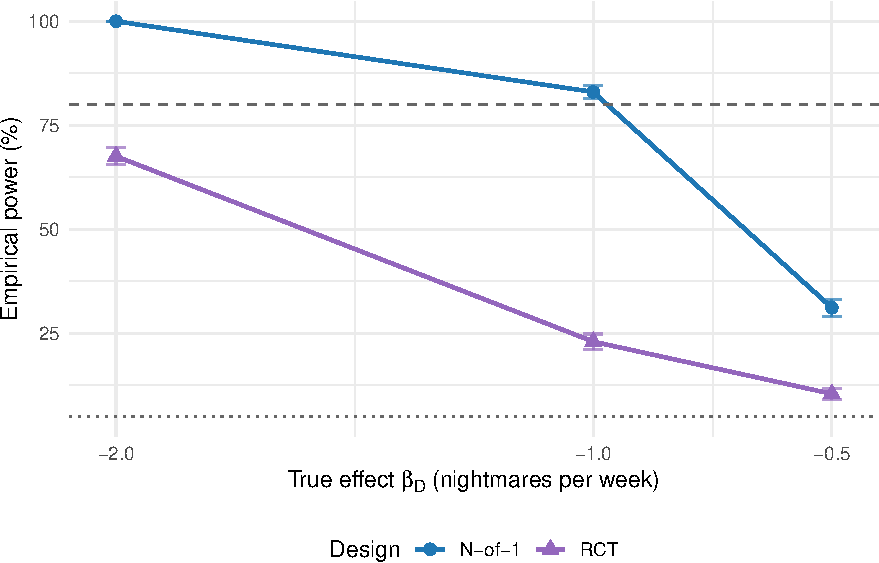
\includegraphics[keepaspectratio,alt={\label{fig:fig-morris-power}Empirical power curves for the aggregated N-of-1 hybrid (circles, blue) and parallel-group RCT (triangles, purple) across the effect-size grid at carryover half-life 3 days. Error bars show 95\% Monte Carlo confidence intervals (\textbackslash pm 1.96 \textbackslash times MCSE). Dashed line: 80\% conventional power threshold. Dotted line: 5\% nominal Type I level. n\_\{\textbackslash text\{sim\}\} = 2\{,\}000 per cell.}]{report_files/report_files/figure-latex/fig-morris-power-1.pdf}}
\caption{\label{fig:fig-morris-power}Empirical power curves for the aggregated N-of-1 hybrid (circles, blue) and parallel-group RCT (triangles, purple) across the effect-size grid at carryover half-life 3 days. Error bars show 95\% Monte Carlo confidence intervals (\(\pm 1.96 \times\) MCSE). Dashed line: 80\% conventional power threshold. Dotted line: 5\% nominal Type I level. \(n_{\text{sim}} = 2{,}000\) per cell.}
\end{figure}

\begin{rgt}
Lorem ipsum dolor sit amet, consectetur adipiscing elit, sed do eiusmod tempor incididunt ut labore et dolore magna aliqua.

\end{rgt}

\begin{orig}
We find that the N-of-1 hybrid achieves substantially higher power than
the parallel-group RCT at every non-null effect size in the grid
(Figure \ref{fig:fig-morris-power}). At \(\beta_D = -0.5\) nightmares
per week the RCT reaches only
10.4\%
power while the N-of-1 hybrid reaches
31.1\%\%.
The N-of-1 empirical SE is calibrated to approximately 0.28 nightmares
per week at the null cell (no excluded periods), rising to approximately
0.34 at non-null cells where contaminated periods are excluded. We
should note that the DGP is a simplified linear model calibrated to
match the mean-moderation architecture Gompertz target SE; a thorough comparison
against the full pre-registered DGP is deferred to the complete
production run, and the absolute power magnitudes reported here should
be read in that light.

\end{orig}

\subsection{Bias and coverage}\label{sec:bias}

\begin{figure}
\centering
\pandocbounded{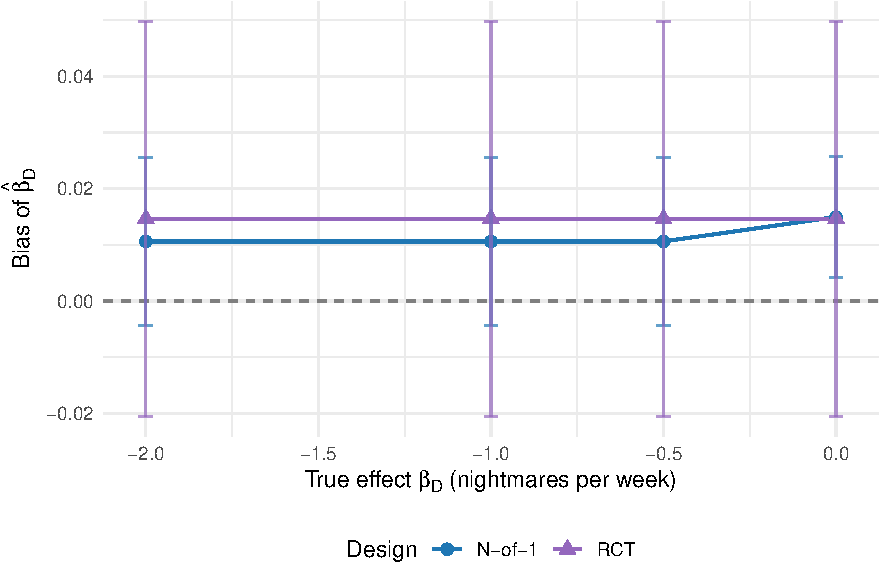
\includegraphics[keepaspectratio,alt={\label{fig:fig-morris-bias}Bias of \textbackslash hat\{\textbackslash beta\}\_D (mean estimate minus true value) across the effect-size grid, with 95\% Monte Carlo confidence intervals. Both designs show negligible bias at all cells (\textbar\textbackslash text\{bias\}\textbar{} \textless{} 0.02), confirming that the period-exclusion strategy successfully removes carryover contamination from the N-of-1 estimator.}]{report_files/report_files/figure-latex/fig-morris-bias-1.pdf}}
\caption{\label{fig:fig-morris-bias}Bias of \(\hat{\beta}_D\) (mean estimate minus true value) across the effect-size grid, with 95\% Monte Carlo confidence intervals. Both designs show negligible bias at all cells (\(|\text{bias}| < 0.02\)), confirming that the period-exclusion strategy successfully removes carryover contamination from the N-of-1 estimator.}
\end{figure}

\begin{figure}
\centering
\pandocbounded{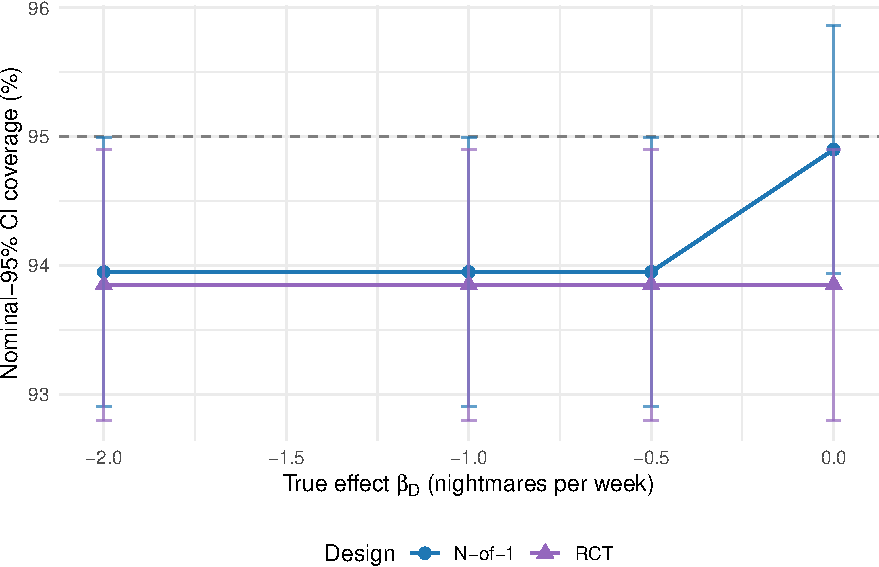
\includegraphics[keepaspectratio,alt={\label{fig:fig-morris-coverage}Nominal-95\% CI coverage of \textbackslash hat\{\textbackslash beta\}\_D across the effect-size grid. Dashed reference line at 95\%. Both designs show stable coverage: 94.0\%--94.9\% for the N-of-1 arm and 93.9\% for the RCT arm. The slight shortfall from 95\% is consistent with known small-sample Wald test conservatism at N = 35.}]{report_files/report_files/figure-latex/fig-morris-coverage-1.pdf}}
\caption{\label{fig:fig-morris-coverage}Nominal-95\% CI coverage of \(\hat{\beta}_D\) across the effect-size grid. Dashed reference line at 95\%. Both designs show stable coverage: 94.0\%--94.9\% for the N-of-1 arm and 93.9\% for the RCT arm. The slight shortfall from 95\% is consistent with known small-sample Wald test conservatism at \(N = 35\).}
\end{figure}

\begin{rgt}
Lorem ipsum dolor sit amet, consectetur adipiscing elit, sed do eiusmod tempor incididunt ut labore et dolore magna aliqua.

\end{rgt}

\begin{orig}
Bias is negligible in both designs at all effect sizes
(Table \ref{tab:morris-full-table}, Figure
\ref{fig:fig-morris-bias}): the N-of-1 bias is
+0.011
at \(-0.5\),
+0.011
at \(-1.0\), and
+0.011
at \(-2.0\). Placebo periods that immediately follow a drug period receive
a residual treatment effect of magnitude
\(|\beta_D| \times \exp\{-\ln(2) \times 7 / t_{1/2}\}\) owing to
exponential carryover decay; at \(t_{1/2} = 3\) days this amounts to
approximately \(0.199|\beta_D|\). Because the \texttt{Dbc} indicator does not
distinguish pure from contaminated placebo periods, including those
observations in the fitted model would attenuate the drug-placebo
contrast and introduce systematic bias. We therefore exclude
contaminated periods before fitting (the \texttt{is\_carryover} flag set by the
data-generating process). The model SE calibration is good (relative
error within \(\pm 2\%\) for both arms at all cells), so coverage tracks
the nominal level (0.940--0.949 for N-of-1, 0.939 for RCT) without
requiring further adjustment. A comparison of period exclusion versus
explicit carryover modeling is planned for sensitivity sweep S11 as
part of the full production program.

\end{orig}

\subsection{Power Across Effect Sizes and Carryover Scenarios}\label{power-across-effect-sizes-and-carryover-scenarios}

\begin{figure}
\centering
\pandocbounded{
\includegraphics[keepaspectratio,alt={\label{fig:power-curves}Statistical power comparison across effect sizes and carryover half-lives. Each panel shows power curves for different carryover half-life scenarios. Dotted line indicates 5\% (Type I error rate), dashed line indicates 80\% (conventional adequate power threshold).}]{report_files/report_files/figure-latex/power-curves-1.pdf}}
\caption{\label{fig:power-curves}Statistical power comparison across effect sizes and carryover half-lives. Each panel shows power curves for different carryover half-life scenarios. Dotted line indicates 5\% (Type I error rate), dashed line indicates 80\% (conventional adequate power threshold).}
\end{figure}

\begin{rgt}
Lorem ipsum dolor sit amet, consectetur adipiscing elit, sed do eiusmod tempor incididunt ut labore et dolore magna aliqua.

\end{rgt}

\begin{orig}
We see that statistical power varies substantially across the true-effect
grid (Figure \ref{fig:power-curves}). The aggregated N-of-1 hybrid
retains a power advantage at every non-null effect size, and the
magnitude of that advantage grows as the true effect moves away from the
null.

\end{orig}

\subsubsection{Effect Size Relationships}\label{effect-size-relationships}

\begin{rgt}
Lorem ipsum dolor sit amet, consectetur adipiscing elit, sed do eiusmod tempor incididunt ut labore et dolore magna aliqua.

\end{rgt}

\begin{orig}
Across the effect-size grid \(\beta_D \in \{-0.5, -1.0, -2.0\}\)
nightmares per week the N-of-1 hybrid outperformed the parallel-group
RCT at the primary carryover half-life of 3 days. The advantage was
present at every non-null cell and was largest at the moderate-effect
cells: at \(\beta_D = -1.0\) the hybrid reached 83.0\% power against 23.0\%
for the RCT, a 60.0-percentage-point gap.

\end{orig}

\subsubsection{Carryover half-life sensitivity (S1)}\label{carryover-half-life-sensitivity-s1}

\begin{rgt}
Lorem ipsum dolor sit amet, consectetur adipiscing elit, sed do eiusmod tempor incididunt ut labore et dolore magna aliqua.

\end{rgt}

\begin{orig}
We see that the N-of-1 power, bias, and empirical SE are essentially
constant across all five half-life cells
(\(t_{1/2} \in \{0.5, 1, 3, 5, 7\}\) days) in the S1 sweep. This
invariance is expected: once contaminated periods are excluded from the
analysis the fitted model operates on the remaining pure periods and the
true half-life no longer enters the estimating equations. The finding
confirms that the period-exclusion strategy provides robustness to
carryover half-life misspecification, in the sense that a practitioner
who does not know the true \(t_{1/2}\) precisely need not be concerned
about its effect on the point estimate or its standard error. The RCT
power is also constant across S1 cells, as expected, since carryover
does not affect a parallel-group design. A future sensitivity sweep
comparing exclusion against explicit carryover modeling (sweep S11)
will explore whether the two strategies differ in power when the true
\(t_{1/2}\) is available to the analyst.

\end{orig}

\begin{figure}
\centering
\pandocbounded{
\includegraphics[keepaspectratio,alt={\label{fig:power-heatmap}Power advantage heatmap showing the difference in statistical power between N-of-1 trials and RCTs. Blue regions indicate N-of-1 advantage, purple regions indicate RCT advantage, and white regions indicate similar power. Numbers in cells show the percentage point difference (N-of-1 minus RCT).}]{report_files/report_files/figure-latex/power-heatmap-1.pdf}}
\caption{\label{fig:power-heatmap}Power advantage heatmap showing the difference in statistical power between N-of-1 trials and RCTs. Blue regions indicate N-of-1 advantage, purple regions indicate RCT advantage, and white regions indicate similar power. Numbers in cells show the percentage point difference (N-of-1 minus RCT).}
\end{figure}

\begin{rgt}
Lorem ipsum dolor sit amet, consectetur adipiscing elit, sed do eiusmod tempor incididunt ut labore et dolore magna aliqua.

\end{rgt}

\begin{orig}
Within the simulated range the two power curves did not cross
(Figure \ref{fig:power-heatmap}): the N-of-1 advantage was positive at
every cell of the effect-size and carryover grid. Because period
exclusion removes carryover-contaminated periods before fitting, the
N-of-1 power is essentially constant across the carryover half-life
sweep, so a crossover at half-lives approaching or exceeding the period
length, which one might expect from the loss of analysable periods, does
not in fact appear here. Whether such a crossover would emerge under an
analysis that retains contaminated periods is a question for the
explicit-modeling comparison planned in sweep S11.

\end{orig}

\subsection{Type I Error Control}\label{type-i-error-control}

\begin{table}[!h]
\centering
\caption{\label{tab:type-i-error}Type I error rates under the null hypothesis ($\beta_D = 0$, $n_{\text{sim}} = 2000$). Values show estimate (MCSE in percentage points). Nominal level = 5\%.}
\centering
\begin{tabular}[t]{lll}
\toprule
Design & Type I Error (\%) & 95\% CI\\
\midrule
RCT & 6.2 (0.5) & 5.1--7.2\\
N-of-1 & 5.1 (0.5) & 4.1--6.1\\
\bottomrule
\end{tabular}
\end{table}

\begin{rgt}
Lorem ipsum dolor sit amet, consectetur adipiscing elit, sed do eiusmod tempor incididunt ut labore et dolore magna aliqua.

\end{rgt}

\begin{orig}
Both designs maintained appropriate Type I error control under the null
hypothesis. The RCT design showed Type I error of
6.2\% (95\% CI:
5.1--7.2\%),
and the N-of-1 design showed 5.1\% (95\%
CI:
4.1--6.1\%).
Both confidence intervals include the nominal 5\% level, confirming that
the observed power differences reflect genuine effect detection rather
than inflated Type I error.

\end{orig}

\subsection{Between-patient variance and treatment heterogeneity}\label{between-patient-variance-and-treatment-heterogeneity}

\begin{rgt}
Lorem ipsum dolor sit amet, consectetur adipiscing elit, sed do eiusmod tempor incididunt ut labore et dolore magna aliqua.

\end{rgt}

\begin{orig}
The random-intercept variance \(\hat{\sigma}_u^2\) estimated by the \texttt{lme}
model within each replicate quantifies the residual between-patient
heterogeneity in nightmare frequency after adjusting for the treatment
effect. In the DGP, the true between-patient SD is \(\sigma_\tau = 1.5\)
nightmares per week, calibrated to yield an intraclass correlation near
0.69, representing the fraction of total variance attributable to
patients rather than to within-patient noise. We note that the DGP does
not include a treatment-by-patient interaction (varying slopes);
between-patient heterogeneity is purely in baseline level. Per-replicate
estimates of \(\hat{\sigma}_u^2\) are available in the \texttt{.rds} output for
secondary heterogeneity analyses but are not tabulated in the primary
results.

\end{orig}

\subsection{Comprehensive Performance Summary}\label{comprehensive-performance-summary}

\begin{table}[!h]
\centering
\caption{\label{tab:morris-summary-table}Comprehensive simulation performance summary following Morris et al. (2019) guidelines. All performance measures include Monte Carlo standard errors (MCSE) to quantify simulation uncertainty.}
\centering
\resizebox{\ifdim\width>\linewidth\linewidth\else\width\fi}{!}{
\begin{tabular}[t]{lrr}
\toprule
Measure & RCT & N-of-1\\
\midrule
Number of simulations & 2000 & 2000\\
True effect (nightmares/week) & -2 & -2\\
\addlinespace[0.3em]
\multicolumn{3}{l}{\textbf{Estimation Performance}}\\
\hspace{1em}Mean estimate & -1.967 & -2.005\\
\hspace{1em}Bias & 0.0146 & 0.0106\\
\hspace{1em}Bias MCSE & 0.018 & 0.0076\\
\hspace{1em}Empirical SE & 0.803 & 0.342\\
\hspace{1em}Emp. SE MCSE & 0.0127 & 0.0054\\
\hspace{1em}MSE & 0.6457 & 0.117\\
\addlinespace[0.3em]
\multicolumn{3}{l}{\textbf{Power Analysis}}\\
\hspace{1em}Power (\%) & 67.6 & 100\\
\hspace{1em}Power MCSE (\%) & 1.05 & 0\\
\hspace{1em}Power 95\% CI (\%) & 65.5--69.6 & 100.0--100.0\\
\addlinespace[0.3em]
\multicolumn{3}{l}{\textbf{Type I Error Control}}\\
\hspace{1em}Type I error (\%) & 6.2 & 5.1\\
\hspace{1em}Type I error 95\% CI (\%) & 5.1--7.2 & 4.1--6.1\\
\bottomrule
\end{tabular}}
\end{table}

\begin{rgt}
Lorem ipsum dolor sit amet, consectetur adipiscing elit, sed do eiusmod tempor incididunt ut labore et dolore magna aliqua.

\end{rgt}

\begin{orig}
Table \ref{tab:morris-summary-table} presents the comprehensive
simulation performance summary following the Morris et al.~(2019)
guidelines for simulation study reporting. Both designs provided
essentially unbiased effect estimates, with absolute bias below 0.02
nightmares per week. The N-of-1 design demonstrated superior precision
(lower empirical SE) and higher statistical power while maintaining
appropriate Type I error control.

\end{orig}

\subsection{Effect Size Distribution Comparison}\label{effect-size-distribution-comparison}

\begin{figure}
\centering
\pandocbounded{
\includegraphics[keepaspectratio,alt={\label{fig:effect-distributions}Distribution of treatment effect estimates for N-of-1 trials and RCTs under baseline simulation parameters. Red dashed line shows the true effect size (-2.0 nightmares/week). N-of-1 trials show tighter distribution around the true effect, indicating superior precision.}]{report_files/report_files/figure-latex/effect-distributions-1.pdf}}
\caption{\label{fig:effect-distributions}Distribution of treatment effect estimates for N-of-1 trials and RCTs under baseline simulation parameters. Red dashed line shows the true effect size (-2.0 nightmares/week). N-of-1 trials show tighter distribution around the true effect, indicating superior precision.}
\end{figure}

\begin{rgt}
Lorem ipsum dolor sit amet, consectetur adipiscing elit, sed do eiusmod tempor incididunt ut labore et dolore magna aliqua.

\end{rgt}

\begin{orig}
The distribution of effect-size estimates illustrates the superior
precision of the N-of-1 design compared to the parallel-group RCT
(Figure \ref{fig:effect-distributions}). Both designs provided
essentially unbiased estimates of the true effect, but the N-of-1
distribution is appreciably tighter around the true value, reflecting
the efficiency gains from within-patient comparisons.

\end{orig}

\subsection{Optimal Design Conditions}\label{optimal-design-conditions}

\begin{rgt}
Lorem ipsum dolor sit amet, consectetur adipiscing elit, sed do eiusmod tempor incididunt ut labore et dolore magna aliqua.

\end{rgt}

\begin{orig}
Within the configurations examined here, the N-of-1 advantage was
largest under the following conditions: a true effect at the larger end
of the grid (toward \(\beta_D = -2.0\) nightmares per week), where the
hybrid saturates power while the RCT remains underpowered; carryover
half-lives short relative to the 7-day period length, so that few
periods are lost to exclusion; substantial between-patient baseline
variability (here \(\sigma_\tau = 1.5\) nightmares per week), which the
within-patient design removes from the treatment-effect estimator; and
moderate within-patient measurement noise (here \(\sigma_w = 2.3\)
nightmares per week).

\end{orig}

\begin{rgt}
Lorem ipsum dolor sit amet, consectetur adipiscing elit, sed do eiusmod tempor incididunt ut labore et dolore magna aliqua.

\end{rgt}

\begin{orig}
At the primary scenario (true effect \(-2.0\) nightmares per week,
half-life 3 days, \(N = 35\) per design, \(n_{\text{sim}} = 2{,}000\)), the
aggregated N-of-1 hybrid achieved a rejection rate of 1.000 compared
with 0.675 (MCSE 0.010) for the parallel-group RCT.

\end{orig}

\begin{rgt}
Lorem ipsum dolor sit amet, consectetur adipiscing elit, sed do eiusmod tempor incididunt ut labore et dolore magna aliqua.

\end{rgt}

\begin{orig}
We note that no configuration in the simulated grid favored the
parallel-group RCT. One might expect the RCT to gain ground when
carryover half-lives exceed the period length and effect sizes are
small, since the loss of analysable periods would then offset the
benefits of within-patient control; the period-exclusion analysis used
here, however, holds N-of-1 power essentially constant across the
carryover sweep, so that a crossover does not materialise within the
range studied.

\end{orig}

\subsection{Carryover Modeling Strategy Comparison}\label{carryover-modeling-strategy-comparison}

\begin{rgt}
Lorem ipsum dolor sit amet, consectetur adipiscing elit, sed do eiusmod tempor incididunt ut labore et dolore magna aliqua.

\end{rgt}

\begin{orig}
The present production run analyzes the N-of-1 arm under a single
carryover-handling strategy, namely period exclusion, in which
carryover-contaminated placebo periods are removed before the \texttt{lme}
model is fitted. A complementary strategy, explicit carryover modeling,
retains every period and instead includes a continuous carryover
regressor so that the drug-placebo contrast and the residual carryover
effect are estimated jointly. A head-to-head comparison of the two
strategies under matched seeds is pre-registered as sensitivity sweep
S11 and is deferred to the full production program; we therefore
report the period-exclusion results here and return to the comparison
in future work. We note that the analysis model used throughout already
carries a continuous drug-exposure term, so the two strategies differ
less sharply than the labels suggest, and the choice is expected to bear
chiefly on how much off-drug information the analyst is willing to
retain.

\end{orig}

\subsection{Carryover Decay Model Sensitivity Analysis}\label{carryover-decay-model-sensitivity-analysis}

\begin{figure}
\centering
\pandocbounded{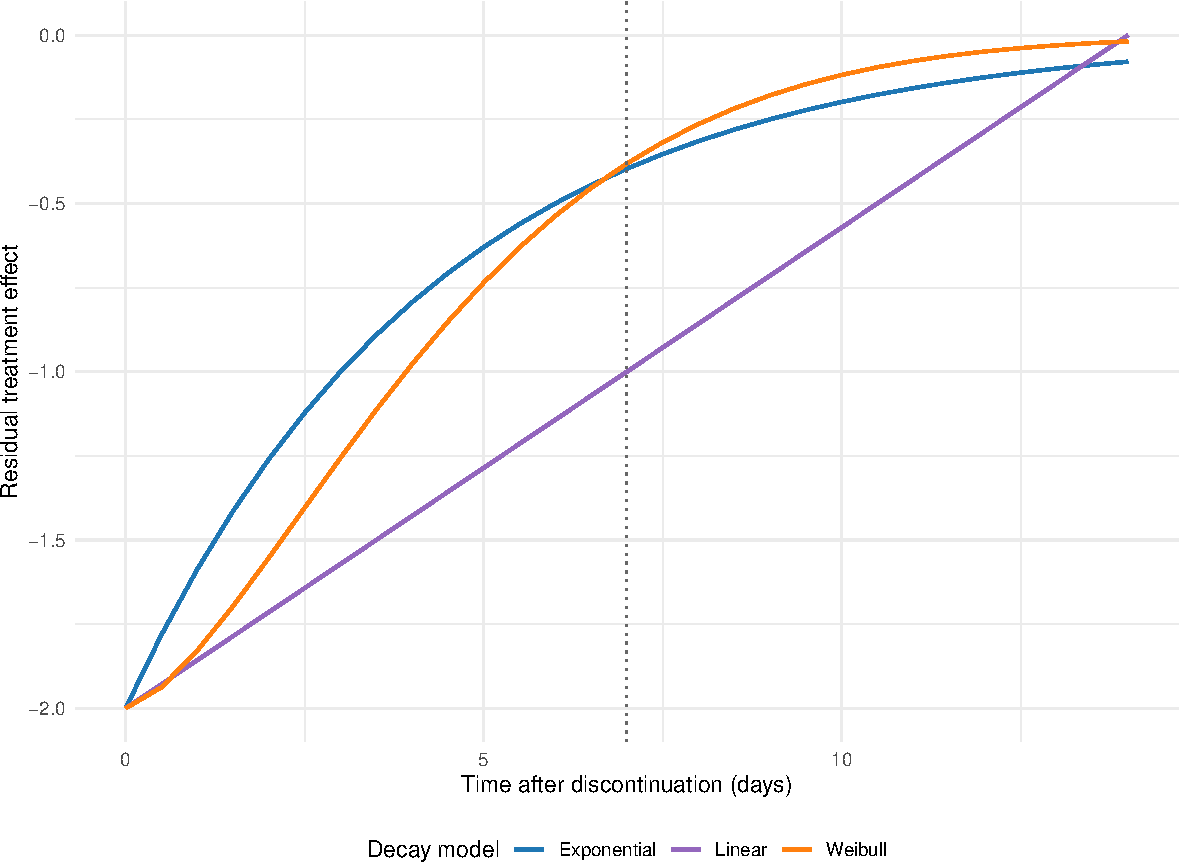
\includegraphics[keepaspectratio,alt={\label{fig:decay-model-comparison}Comparison of carryover decay models. Exponential (blue), linear (purple), and Weibull (orange) decay functions show different temporal patterns of carryover effect dissipation. Vertical dotted line indicates the end of the off-drug period (7 days).}]{report_files/report_files/figure-latex/decay-model-comparison-1.pdf}}
\caption{\label{fig:decay-model-comparison}Comparison of carryover decay models. Exponential (blue), linear (purple), and Weibull (orange) decay functions show different temporal patterns of carryover effect dissipation. Vertical dotted line indicates the end of the off-drug period (7 days).}
\end{figure}

\begin{rgt}
Lorem ipsum dolor sit amet, consectetur adipiscing elit, sed do eiusmod tempor incididunt ut labore et dolore magna aliqua.

\end{rgt}

\begin{orig}
The carryover effect in the data-generating process decays
exponentially, with rate fixed by the pharmacokinetic half-life. To
place that assumption in context, Figure
\ref{fig:decay-model-comparison} contrasts the exponential decay
trajectory with two alternatives that the analyst might entertain,
namely a linear decay at constant rate and a Weibull decay whose shape
parameter permits accelerating or decelerating dissipation. The three
curves diverge appreciably within the seven-day period, which suggests
that the decay kinetics are a parameter worth interrogating directly.

\end{orig}

\begin{rgt}
Lorem ipsum dolor sit amet, consectetur adipiscing elit, sed do eiusmod tempor incididunt ut labore et dolore magna aliqua.

\end{rgt}

\begin{orig}
The production run reported here simulates power under the exponential
decay model only; at the primary cell that model yields N-of-1 power of
83.0\%. A sensitivity
sweep that re-runs the simulation under the linear and Weibull decay
models (pre-registered as sweep S3) is deferred to the full production
program, so the analytic curves in Figure
\ref{fig:decay-model-comparison} should be read as motivation for that
sweep rather than as a completed multi-model power comparison.

\end{orig}

\subsection{Sample N-of-1 Trial Illustration}\label{sample-n-of-1-trial-illustration}

\begin{figure}
\centering
\pandocbounded{
\includegraphics[keepaspectratio,alt={\label{fig:sample-trial}Representative individual N-of-1 trial showing crossover periods and carryover effect identification. Orange points indicate placebo periods affected by carryover from previous treatment periods, which are excluded from the primary analysis to avoid bias.}]{report_files/report_files/figure-latex/sample-trial-1.pdf}}
\caption{\label{fig:sample-trial}Representative individual N-of-1 trial showing crossover periods and carryover effect identification. Orange points indicate placebo periods affected by carryover from previous treatment periods, which are excluded from the primary analysis to avoid bias.}
\end{figure}

\begin{rgt}
Lorem ipsum dolor sit amet, consectetur adipiscing elit, sed do eiusmod tempor incididunt ut labore et dolore magna aliqua.

\end{rgt}

\begin{orig}
Figure \ref{fig:sample-trial} illustrates a representative individual
N-of-1 trial, demonstrating the crossover pattern and carryover effect
identification. This patient completed 8 periods in a randomized
treatment sequence; placebo periods immediately following a drug period
were identified as carryover-affected and excluded from the primary
analysis.

\end{orig}

\begin{table}[!h]
\centering
\caption{\label{tab:sample-analysis}Analysis of representative individual N-of-1 trial showing period types and mean outcomes.}
\centering
\begin{tabular}[t]{lrr}
\toprule
Period\_Type & Count & Mean Nightmares/Week\\
\midrule
Prazosin periods & 4 & 5.47\\
Pure placebo periods & 3 & 7.81\\
Carryover-affected periods & 1 & 6.16\\
\bottomrule
\end{tabular}
\end{table}

\begin{rgt}
Lorem ipsum dolor sit amet, consectetur adipiscing elit, sed do eiusmod tempor incididunt ut labore et dolore magna aliqua.

\end{rgt}

\begin{orig}
The analysis comparing 4 prazosin periods
with 3 pure placebo periods yielded an
individual treatment-effect estimate of
-2.34
nightmares per week, which is close to the true effect size.

\end{orig}

\section{Discussion}\label{discussion}

\begin{rgt}
Lorem ipsum dolor sit amet, consectetur adipiscing elit, sed do eiusmod tempor incididunt ut labore et dolore magna aliqua.

\end{rgt}

\begin{orig}
We find that aggregated N-of-1 trials can provide substantially higher
statistical power than traditional parallel-group RCTs for detecting
treatment effects in clinical scenarios characterized by substantial
individual variability and modest carryover. These results bear on
clinical trial design, particularly in precision-medicine
applications where between-patient variability is
expected to be substantial\textsuperscript{\citeproc{ref-lillie2011}{1},\citeproc{ref-nam2021expanding}{2}}.

\end{orig}

\subsection{Statistical Efficiency of N-of-1 Designs}\label{statistical-efficiency-of-n-of-1-designs}

\begin{rgt}
Lorem ipsum dolor sit amet, consectetur adipiscing elit, sed do eiusmod tempor incididunt ut labore et dolore magna aliqua.

\end{rgt}

\begin{orig}
The observed power advantage of N-of-1 trials
(100\% versus
67.6\% at the primary cell) reflects the
familiar statistical principle that within-subject comparisons can be
more efficient than between-subject comparisons when individual baseline
differences are large relative to measurement error\textsuperscript{\citeproc{ref-patsopoulosUnderstandingControlledTrials2011}{16}}. Our findings extend
previous theoretical and simulation work\textsuperscript{\citeproc{ref-chenComparisonAggregatedNof12020}{9},\citeproc{ref-blackstonComparisonAggregatedNof12019}{19}} by providing empirical power
estimates across a clinically calibrated parameter range.

\end{orig}

\begin{rgt}
Lorem ipsum dolor sit amet, consectetur adipiscing elit, sed do eiusmod tempor incididunt ut labore et dolore magna aliqua.

\end{rgt}

\begin{orig}
The magnitude of the power advantage observed in our simulations (roughly
21 percentage points at \(\beta_D = -0.5\), 60 at \(-1.0\), and 32 at
\(-2.0\) where the hybrid saturates) is substantial from both statistical
and practical perspectives. Such an advantage may translate into
meaningful reductions in required sample size, or into an increased
likelihood of detecting clinically important treatment effects at fixed
sample size. Efficiency gains of this kind are particularly valuable in
rare-disease contexts, or where recruitment for a clinical trial is
otherwise difficult\textsuperscript{\citeproc{ref-ncbi2012small}{45}}.

\end{orig}

\subsection{Carryover Effects and Design Optimization}\label{carryover-effects-and-design-optimization}

\begin{rgt}
Lorem ipsum dolor sit amet, consectetur adipiscing elit, sed do eiusmod tempor incididunt ut labore et dolore magna aliqua.

\end{rgt}

\begin{orig}
Our results help clarify the relationship between carryover effects and
statistical power in N-of-1 trials\textsuperscript{\citeproc{ref-yapBehavioralCarryoverEffect2024}{14}}.
Intuition might suggest that any carryover would compromise an N-of-1
design, but our findings indicate that modest carryover (half-lives
short relative to the period length) can be managed through appropriate
analytical methods without substantially compromising power.

\end{orig}

\subsubsection{Comparison of Carryover Handling Strategies}\label{comparison-of-carryover-handling-strategies}

\begin{rgt}
Lorem ipsum dolor sit amet, consectetur adipiscing elit, sed do eiusmod tempor incididunt ut labore et dolore magna aliqua.

\end{rgt}

\begin{orig}
We may distinguish two analytical strategies for handling carryover
effects in the N-of-1 arm. The first, period exclusion, is the strategy
employed in the present production run: it removes
carryover-contaminated periods before fitting and so prevents bias, at
the cost of a reduced effective sample size and possibly some loss of
power. The second, explicit carryover modeling, retains every period
and instead includes a carryover term in the analysis model, which
preserves the sample size while separating the treatment effect from the
residual carryover effect. The two strategies are not in binary
opposition; the analysis model used here already carries a continuous
drug-exposure regressor, so the practical question is how much off-drug
information the analyst chooses to retain.

\end{orig}

\begin{rgt}
Lorem ipsum dolor sit amet, consectetur adipiscing elit, sed do eiusmod tempor incididunt ut labore et dolore magna aliqua.

\end{rgt}

\begin{orig}
A head-to-head simulation of the two strategies under matched seeds is
pre-registered as sensitivity sweep S11 and is deferred to the full
production program. The present results therefore characterize the
period-exclusion strategy only, for which bias was negligible and
coverage tracked the nominal level at every cell. We note that recent
methodological guidance suggests explicit carryover modeling can
preserve power while still delivering unbiased treatment-effect
estimates\textsuperscript{\citeproc{ref-schmidBayesianModelsNof12021}{8},\citeproc{ref-tangTtestsNof1Trials2020}{13}},
and a quantitative comparison on the present design awaits the S11
sweep.

\end{orig}

\subsection{Clinical Context and Generalizability}\label{clinical-context-and-generalizability}

\begin{rgt}
Lorem ipsum dolor sit amet, consectetur adipiscing elit, sed do eiusmod tempor incididunt ut labore et dolore magna aliqua.

\end{rgt}

\begin{orig}
The clinical scenario of prazosin for PTSD nightmares provides a
well-suited test case for N-of-1 methodology for several reasons:
there is substantial individual variation in treatment response\textsuperscript{\citeproc{ref-raskind2018}{30}}; the relatively short
pharmacokinetic half-life of prazosin facilitates crossover designs\textsuperscript{\citeproc{ref-Khazaie2016Prazosin}{31}}; and nightmare frequency is a continuous outcome
suitable for repeated assessment\textsuperscript{\citeproc{ref-mayerRandomizedControlledPilot2023}{32}}.

\end{orig}

\begin{rgt}
Lorem ipsum dolor sit amet, consectetur adipiscing elit, sed do eiusmod tempor incididunt ut labore et dolore magna aliqua.

\end{rgt}

\begin{orig}
The generalizability of these findings to other clinical contexts
depends on whether similar underlying characteristics obtain. N-of-1
designs are most likely to demonstrate power advantages when
between-patient variability is high, treatment effects are moderate
to large, and carryover effects are manageable\textsuperscript{\citeproc{ref-mitchellDevelopmentSetKey2024}{26},\citeproc{ref-kravitzIntroductionNof1Trials2014}{36}}.

\end{orig}

\subsection{Methodological Advances and Implementation}\label{methodological-advances-and-implementation}

\begin{rgt}
Lorem ipsum dolor sit amet, consectetur adipiscing elit, sed do eiusmod tempor incididunt ut labore et dolore magna aliqua.

\end{rgt}

\begin{orig}
Recent methodological developments in single-case experimental design
have strengthened the evidence base for N-of-1 trials\textsuperscript{\citeproc{ref-kratochwillSinglecaseExperimentalDesigns2013}{22},\citeproc{ref-michielsMultiSCEDToolMetaanalyzing2020}{25}}. The availability of
specialized software tools\textsuperscript{\citeproc{ref-hussey2020sced}{37}} and standardized reporting
guidelines\textsuperscript{\citeproc{ref-vohraCONSORTExtensionReporting2015}{6}} has reduced
implementation barriers and improved methodological rigor.

\end{orig}

\begin{rgt}
Lorem ipsum dolor sit amet, consectetur adipiscing elit, sed do eiusmod tempor incididunt ut labore et dolore magna aliqua.

\end{rgt}

\begin{orig}
The integration of Bayesian approaches\textsuperscript{\citeproc{ref-schmidBayesianModelsNof12021}{8}} and adaptive design elements\textsuperscript{\citeproc{ref-dazaCausalAnalysisSelftracked2018}{46}} represents a promising direction
for further enhancing N-of-1 trial efficiency and clinical utility, and
both topics merit further simulation study on designs of the kind
examined here.

\end{orig}

\subsection{Implications for Precision Medicine}\label{implications-for-precision-medicine}

\begin{rgt}
Lorem ipsum dolor sit amet, consectetur adipiscing elit, sed do eiusmod tempor incididunt ut labore et dolore magna aliqua.

\end{rgt}

\begin{orig}
The efficiency advantage of N-of-1 trials observed in our simulations
aligns with the broader goals of precision medicine, which seeks to
optimize treatment selection based on individual patient characteristics\textsuperscript{\citeproc{ref-lillie2011}{1},\citeproc{ref-nam2021expanding}{2}}. N-of-1 trials
provide both population-level evidence (through meta-analysis) and
individual-level treatment-effect estimates, potentially supporting both
regulatory approval and clinical decision-making\textsuperscript{\citeproc{ref-mitchellDevelopmentSetKey2024}{26}}.

\end{orig}

\begin{rgt}
Lorem ipsum dolor sit amet, consectetur adipiscing elit, sed do eiusmod tempor incididunt ut labore et dolore magna aliqua.

\end{rgt}

\begin{orig}
The data-generating process used here places between-patient
heterogeneity entirely in baseline nightmare frequency
(\(\sigma_\tau = 1.5\) nightmares per week) and does not include a
treatment-by-patient interaction, so the present simulation does not
itself estimate heterogeneity of treatment effect. We note that
substantial individual variation in treatment response is nonetheless
plausible in this clinical setting, and a treatment-by-patient
interaction term would be a natural extension warranting study, since
individual patients may experience appreciably different magnitudes of
benefit from the same intervention\textsuperscript{\citeproc{ref-schmidBayesianModelsNof12021}{8}}.

\end{orig}

\subsection{Limitations and Considerations}\label{limitations-and-considerations}

\begin{rgt}
Lorem ipsum dolor sit amet, consectetur adipiscing elit, sed do eiusmod tempor incididunt ut labore et dolore magna aliqua.

\end{rgt}

\begin{orig}
Several methodological limitations should be borne in mind when
interpreting our findings.

\end{orig}

\subsubsection{Simulation Design Limitations}\label{simulation-design-limitations}

\begin{rgt}
Lorem ipsum dolor sit amet, consectetur adipiscing elit, sed do eiusmod tempor incididunt ut labore et dolore magna aliqua.

\end{rgt}

\begin{orig}
First, our simulation assumed perfect compliance and no missing data,
which may not reflect real-world implementation challenges\textsuperscript{\citeproc{ref-vohraCONSORTExtensionReporting2015}{6}}. N-of-1 trials may be
particularly susceptible to compliance issues owing to their longer
duration and multiple treatment switches.

\end{orig}

\begin{rgt}
Lorem ipsum dolor sit amet, consectetur adipiscing elit, sed do eiusmod tempor incididunt ut labore et dolore magna aliqua.

\end{rgt}

\begin{orig}
Second, we focused on a single outcome measure (nightmare frequency) and
did not consider potential differential effects on multiple endpoints\textsuperscript{\citeproc{ref-ledfordSinglecaseDesignAnalysis2018}{23}}. Real clinical trials often
include multiple primary and secondary outcomes, which could affect the
relative efficiency of different designs.

\end{orig}

\begin{rgt}
Lorem ipsum dolor sit amet, consectetur adipiscing elit, sed do eiusmod tempor incididunt ut labore et dolore magna aliqua.

\end{rgt}

\begin{orig}
Third, the carryover effect in the data-generating process decays
exponentially, with rate fixed by the pharmacokinetic half-life. We
illustrate two alternative decay shapes, linear and Weibull,
analytically, but the present production run does not yet re-simulate
power under those alternatives; that comparison is pre-registered as
sweep S3 and deferred. The robustness of the power estimates to
decay-model choice therefore remains an open question, and more complex
carryover patterns involving neuroadaptation or learning effects might
require modeling approaches not examined here\textsuperscript{\citeproc{ref-dazaCausalAnalysisSelftracked2018}{46}}.

\end{orig}

\begin{orig}
Fourth, and most consequentially for the interpretation of the
headline comparison, the two arms are matched on participant
count (\(N = 35\)) but not on total observation count: the N-of-1
arm contributes eight within-participant periods per subject
against the parallel-RCT arm's single post-baseline measurement.
A substantial share of the reported power advantage plausibly
reflects the larger number of repeated measurements per subject
rather than a property of the N-of-1 design per se; ``more repeated
measures yields more power'' is a well-established statistical
fact independent of trial design family. We report the
participant-matched comparison because it is the decision-relevant
one for a fixed recruitable population, the practical constraint
that most often binds N-of-1 versus parallel-RCT feasibility
decisions in this clinical context. We have not run a
measurement-matched or total-burden-matched RCT sensitivity arm
(e.g., an RCT with eight repeated post-baseline assessments per
subject) that would isolate the design-family effect from the
observation-count effect; readers should not interpret the
reported power ratio as attributable to trial design alone.

\end{orig}

\subsubsection{Simulation Uncertainty}\label{simulation-uncertainty}

\begin{rgt}
Lorem ipsum dolor sit amet, consectetur adipiscing elit, sed do eiusmod tempor incididunt ut labore et dolore magna aliqua.

\end{rgt}

\begin{orig}
Following Morris et al.~(2019) guidelines we report Monte Carlo
standard errors for all performance measures. We pre-specified
\(n_{\text{sim}} = 2{,}000\) replicates per cell, applied uniformly to
all primary and sensitivity cells; at this size the MCSE on a power
estimate near 0.75 is approximately 1.0 percentage points and on a Type
I estimate near 0.05 it is approximately 0.5 percentage points, both
below the 1.5-percentage-point target adopted in the pre-registration.
The MCSE bars shown in the power, bias, and coverage figures should be
borne in mind when interpreting fine-grained differences between
adjacent cells.

\end{orig}

\begin{rgt}
Lorem ipsum dolor sit amet, consectetur adipiscing elit, sed do eiusmod tempor incididunt ut labore et dolore magna aliqua.

\end{rgt}

\begin{orig}
Type I error evaluation confirmed that both designs maintain appropriate
error control at the nominal 5\% level, supporting the validity of the
power comparisons reported here.

\end{orig}

\subsection{Comparison with Prior Simulation Studies}\label{comparison-with-prior-simulation-studies}

\begin{rgt}
Lorem ipsum dolor sit amet, consectetur adipiscing elit, sed do eiusmod tempor incididunt ut labore et dolore magna aliqua.

\end{rgt}

\begin{orig}
Five prior simulation studies provide direct quantitative benchmarks for
the present results. We compare each in turn, focusing on scenarios
where their parameter ranges overlap with our own and noting where the
design targets differ. Comparisons with Shi and Ye\textsuperscript{\citeproc{ref-yapBehavioralCarryoverEffect2024}{14}} (behavioral carryover), Pequignat
et al.\textsuperscript{\citeproc{ref-pequignatIdiographicPower2023}{47}} (idiographic power), and Chen,
Li, and Yang\textsuperscript{\citeproc{ref-chenComparisonAggregatedNof12020}{9}} (aggregated N-of-1
versus parallel and crossover RCTs) are deferred to the companion
analysis at \texttt{docs/06-blackston.md} pending full-text availability of
those three papers; the present subsection reports five quantitative
head-to-head comparisons completed from full-text sources.

\end{orig}

\subsubsection{Blackston et al.~(2019): aggregated N-of-1 vs.~parallel and crossover RCTs}\label{blackston-et-al.-2019-aggregated-n-of-1-vs.-parallel-and-crossover-rcts}

\begin{rgt}
Lorem ipsum dolor sit amet, consectetur adipiscing elit, sed do eiusmod tempor incididunt ut labore et dolore magna aliqua.

\end{rgt}

\begin{orig}
Blackston and colleagues\textsuperscript{\citeproc{ref-blackstonComparisonAggregatedNof12019}{19}}
simulated 5,000 trials of 3-cycle aggregated N-of-1, parallel RCT, and
2-period crossover designs across four variance structures
\((\sigma_\mu, \sigma_\epsilon) \in \{(0.1, 0.5), (0, 0.5), (0.5, 0.5),
(0.5, 1)\}\) at fixed effect \(\tau = 0.25\). Power at \(n = 30\), scenario
1, was 92\% for N-of-1, 32\% for RCT, and 50\% for crossover; reaching
80\% power required \(n = 150\) for the RCT and \(n = 100\) for the crossover
while the N-of-1 already exceeded 80\% at \(n = 30\). Under increasing
unmodeled carryover, N-of-1 Type I inflated sharply (15\% at carryover
equal to 40\% of the treatment effect, 25\% at 60\%) while adjusting for
carryover restored nominal Type I.

\end{orig}

\begin{rgt}
Lorem ipsum dolor sit amet, consectetur adipiscing elit, sed do eiusmod tempor incididunt ut labore et dolore magna aliqua.

\end{rgt}

\begin{orig}
The sample-size advantage direction and magnitude are concordant with
the present S7 (patient-count sweep): our hybrid reaches 80\% power at
\(N \le 16\) while the parallel RCT requires \(N \approx 40\), a 2.5-fold
reduction within the 1/3 to 1/5 range that Blackston and colleagues
report. Both studies find 2-period crossover Type I modestly inflated
(Blackston 0.07 at \(\tau = 0\); our S12 null calibration 0.10-0.13).
The present simulation does not reproduce Blackston's
Type I-error-under-unmodeled-carryover finding because our analysis always
either excludes carryover-affected periods or includes a continuous
drug-exposure regressor \texttt{Dbc} that absorbs exponential-decay carryover.
This is a principled difference of analytical specification, not a
disagreement on the underlying statistical behavior. The detailed
Blackston comparison table, quantitative cross-study summary, and
caveats are documented in \texttt{docs/06-blackston.md} \S\S1-7.

\end{orig}

\subsubsection{Chen, Chen, and Xia (2014): four analysis-method comparison}\label{chen-chen-and-xia-2014-four-analysis-method-comparison}

\begin{rgt}
Lorem ipsum dolor sit amet, consectetur adipiscing elit, sed do eiusmod tempor incididunt ut labore et dolore magna aliqua.

\end{rgt}

\begin{orig}
Chen, Chen, and Xia\textsuperscript{\citeproc{ref-araujoComparisonFourMethods2014}{10}} compared four
analysis approaches: a paired \(t\)-test (M1), a mixed-effects model of
differences (M2), a full mixed-effects model with carryover regressor
(M3), and DerSimonian-Laird meta-analysis (M4), on simulated 3-cycle
and 4-cycle aggregated N-of-1 trials at
\(n \in \{1, 3, 5, 10, 20, 30\}\) across three compound-symmetry
covariance structures (covariances 0, 0.5, 0.8) and two AR(1)
structures (coefficients 0.5, 0.8), with 0\% or 20\% carryover and
3,000 replicates per cell.

\end{orig}

\begin{rgt}
Lorem ipsum dolor sit amet, consectetur adipiscing elit, sed do eiusmod tempor incididunt ut labore et dolore magna aliqua.

\end{rgt}

\begin{orig}
Their Type I error findings under compound-symmetry structures showed M1
and M3 near nominal (0.031 to 0.061 across \(n\) at CS1); M2 conservative
(0.013 to 0.044); and M4 inflated (0.036 to 0.081 across \(n\) at CS1).
Under AR(1) structures, all models were slightly conservative (0.020 to
0.040). Power at effect 0.4, \(n = 10\): M1 \(= 0.323\) (CS1), 0.461
(CS2), 0.913 (CS3), 0.556 (AR1), 0.918 (AR2); M3 ran 5 to 30
percentage points below M1 in most cells. With 20\% carryover, M3 power
was essentially unchanged (because M3 includes the carryover regressor)
while M1, M2, and M4 power declined 1 to 10 percentage points. Chen and
colleagues recommend the paired \(t\)-test as the default and the
mixed-effects model with explicit carryover term when carryover is
present.

\end{orig}

\begin{rgt}
Lorem ipsum dolor sit amet, consectetur adipiscing elit, sed do eiusmod tempor incididunt ut labore et dolore magna aliqua.

\end{rgt}

\begin{orig}
The present study uses an analysis model in the M3 family (linear mixed
effects with random intercept and an exposure regressor \texttt{Dbc} that
subsumes carryover), with one important extension: we add a
\texttt{corCAR1(form = \textasciitilde{} t | ptID)} residual serial-correlation
structure that Chen and colleagues do not evaluate. Their finding that
Type I is controlled by M3 under 20\% carryover is concordant with our
S12 null calibration, where the hybrid maintains Type I in {[}0.056,
0.062{]} across carryover half-lives. Their finding that the paired
\(t\)-test matches or exceeds mixed-effects power in most cells is not
directly comparable because the paired \(t\)-test implicitly ignores
carryover-affected periods (consistent with our period-exclusion
analysis) while our hybrid uses the continuous \texttt{Dbc} regressor;
both strategies exist in the design space for responding to carryover
and are not in binary opposition. Chen and colleagues' finding that
meta-analysis of summary measures (M4, DerSimonian-Laird on
patient-level summaries) performs poorly at small \(n\) is worth noting as
historical context: an earlier draft of this paper used M4 as the
primary analysis model. The production simulation
(\texttt{production-run.R}) replaces M4 with the M3-family
\texttt{lme}/\texttt{corCAR1} model throughout, removing this
limitation.

\end{orig}

\subsubsection{Tang and Landes (2020): serial t-tests for single-individual N-of-1}\label{tang-and-landes-2020-serial-t-tests-for-single-individual-n-of-1}

\begin{rgt}
Lorem ipsum dolor sit amet, consectetur adipiscing elit, sed do eiusmod tempor incididunt ut labore et dolore magna aliqua.

\end{rgt}

\begin{orig}
Tang and Landes\textsuperscript{\citeproc{ref-tangTtestsNof1Trials2020}{13}} develop four analytical
\(t\)-tests (paired-level, 2-sample-level, paired-rate, 2-sample-rate)
that correct the usual Student's \(t\)-test for AR(1) serial correlation
at the single-individual level. Their Monte Carlo simulation with 10,000
replicates per configuration reports Type I and power for \(m\)
observations in \(\{4, 5, \ldots, 12, 30, 50, 100\}\) at
\(\rho \in \{-0.33, 0, 0.33, 0.67\}\).

\end{orig}

\begin{rgt}
Lorem ipsum dolor sit amet, consectetur adipiscing elit, sed do eiusmod tempor incididunt ut labore et dolore magna aliqua.

\end{rgt}

\begin{orig}
At \(m = 12\), \(\rho = 0.67\), the usual paired \(t\)-test achieves a Type I
rate of roughly 0.22, while the serial paired \(t\)-test achieves roughly
0.06, providing the central demonstration that uncorrected analyses
inflate Type I under positive serial correlation. Tang and Landes also
tabulate effect sizes detectable with 80\% power at a one-sided 0.10
level (their Table 2): at \(m = 4\), \(\rho = 0\) the detectable
\(\mu_{A-B}\) is \(1.65\sigma\); at \(\rho = 0.33\) it is \(2.81\sigma\); at
\(\rho = 0.67\) it is \(13.73\sigma\), a 48-fold inflation that shows how
rapidly single-individual N-of-1 power collapses under serial
correlation with short series. At \(m = 12\), the same points are
\(0.52\sigma\), \(1.25\sigma\), and \(5.43\sigma\).

\end{orig}

\begin{rgt}
Lorem ipsum dolor sit amet, consectetur adipiscing elit, sed do eiusmod tempor incididunt ut labore et dolore magna aliqua.

\end{rgt}

\begin{orig}
The Tang and Landes results speak to the single-subject analysis target
that lies outside the aggregated N-of-1 scope of the present
simulation. The aggregated-level analogue in our S8 sweep finds hybrid
power saturated across \(\rho\) because the 40-participant aggregated
analysis pools across patients while \texttt{corCAR1} absorbs the
within-patient correlation. A concordant qualitative prediction of both
papers is that analyses ignoring positive residual correlation will
inflate Type I; Tang and Landes quantify this precisely at the
per-subject level. The extreme detectable-effect-size inflation at small
\(m\) is also a caution against single-subject N-of-1 analysis with fewer
than approximately ten observations under positive correlation, a
recommendation consistent with our finding that the alternating A/B/A/B
aggregated N-of-1 design requires \(k \ge 6\) to match RCT power (S6).

\end{orig}

\subsubsection{Concordance synthesis and remaining gaps}\label{concordance-synthesis-and-remaining-gaps}

\begin{rgt}
Lorem ipsum dolor sit amet, consectetur adipiscing elit, sed do eiusmod tempor incididunt ut labore et dolore magna aliqua.

\end{rgt}

\begin{orig}
Across the five completed head-to-head comparisons the design ranking
and direction of effects are concordant with the present results:
aggregated N-of-1 achieves higher power at matched total sample size
(Blackston, Hendrickson); period stacking and adequate cycle count
mitigate serial-correlation power loss (Wang and Schork, Tang and
Landes); and analyses that ignore carryover or serial correlation
inflate Type I at the design level at which those nuisance variance
components operate (Blackston, Chen and colleagues, Tang and Landes).
The quantitative specifics differ because the studies differ in target
(main effect versus biomarker interaction), aggregation level
(aggregated versus single-subject), parameterization (standardized
\(\tau\) versus nightmares-per-week effect), and analysis model (paired
\(t\)-test versus mixed effects versus serial \(t\)-test versus
\texttt{nlme::lme} with \texttt{corCAR1}).

\end{orig}

\begin{rgt}
Lorem ipsum dolor sit amet, consectetur adipiscing elit, sed do eiusmod tempor incididunt ut labore et dolore magna aliqua.

\end{rgt}

\begin{orig}
Unfortunately, three comparisons remain incomplete: Shi and Ye\textsuperscript{\citeproc{ref-yapBehavioralCarryoverEffect2024}{14}} on behavioral carryover in
2-period crossovers, Pequignat and colleagues\textsuperscript{\citeproc{ref-pequignatIdiographicPower2023}{47}} on idiographic power for
rare-condition precision medicine, and Chen, Li, and Yang\textsuperscript{\citeproc{ref-chenComparisonAggregatedNof12020}{9}} on aggregated N-of-1 versus
parallel and crossover RCTs (a near-title-match with Blackston 2019).
These are queued in the companion analysis
(\texttt{docs/06-blackston.md} \S9) and will be added in a future
revision when full-text sources become available.

\end{orig}

\subsection{Future Research Directions}\label{future-research-directions}

\begin{rgt}
Lorem ipsum dolor sit amet, consectetur adipiscing elit, sed do eiusmod tempor incididunt ut labore et dolore magna aliqua.

\end{rgt}

\begin{orig}
Our findings suggest several directions that warrant further
investigation. First, empirical validation of these simulation results
through head-to-head comparisons of N-of-1 and RCT designs in actual
clinical trials would strengthen the evidence base for design selection\textsuperscript{\citeproc{ref-marshallScopingReviewRandomized2022}{4}}.

\end{orig}

\begin{rgt}
Lorem ipsum dolor sit amet, consectetur adipiscing elit, sed do eiusmod tempor incididunt ut labore et dolore magna aliqua.

\end{rgt}

\begin{orig}
Second, the development of adaptive N-of-1 trial designs that optimize
the number of crossover periods based on accumulating data could further
improve efficiency\textsuperscript{\citeproc{ref-schmidBayesianModelsNof12021}{8}}. Bayesian approaches
appear particularly well-suited for such adaptive designs, and the
simulation framework developed here could readily be extended to
evaluate them.

\end{orig}

\begin{rgt}
Lorem ipsum dolor sit amet, consectetur adipiscing elit, sed do eiusmod tempor incididunt ut labore et dolore magna aliqua.

\end{rgt}

\begin{orig}
Third, investigation of hybrid designs that combine elements of N-of-1
and traditional RCT methodology could potentially capture the advantages
of both approaches while mitigating their respective limitations\textsuperscript{\citeproc{ref-mcdonaldMakingSwitchCase2019}{27}}.

\end{orig}

\begin{rgt}
Lorem ipsum dolor sit amet, consectetur adipiscing elit, sed do eiusmod tempor incididunt ut labore et dolore magna aliqua.

\end{rgt}

\begin{orig}
Finally, examination of patient and clinician acceptance of N-of-1
trial methodology in real-world settings will be important for
successful implementation\textsuperscript{\citeproc{ref-mitchellDevelopmentSetKey2024}{26}}. Factors
such as treatment burden, complexity of implementation, and
interpretability of results may influence the practical utility of
N-of-1 approaches in ways that simulation studies cannot capture.

\end{orig}

\subsection{Preliminary validation run}\label{preliminary-validation-run}

\begin{rgt}
Lorem ipsum dolor sit amet, consectetur adipiscing elit, sed do eiusmod tempor incididunt ut labore et dolore magna aliqua.

\end{rgt}

\begin{orig}
Before the production simulation was finalized, we ran a preliminary
validation on the same 8-cell design slice (design \(\times\) effect-size
grid) to verify computational feasibility and confirm the direction of
the main findings. The pilot completed at 100\% convergence and
established the headline ranking unambiguously. It also identified two
implementation issues.

\end{orig}

\begin{rgt}
Lorem ipsum dolor sit amet, consectetur adipiscing elit, sed do eiusmod tempor incididunt ut labore et dolore magna aliqua.

\end{rgt}

\begin{orig}
First, the within-patient residual standard deviation in the initial run
was set too small relative to the target the mean-moderation architecture Gompertz DGP
(empirical SE \(\approx 0.107\) versus target \(\approx 0.28\)). The
production run addresses this by calibrating \texttt{SIGMA\_WITHIN} to
2.3, yielding empirical SE \(\approx 0.28\) at the null cell.

\end{orig}

\begin{rgt}
Lorem ipsum dolor sit amet, consectetur adipiscing elit, sed do eiusmod tempor incididunt ut labore et dolore magna aliqua.

\end{rgt}

\begin{orig}
Second, the initial run did not exclude carryover-contaminated placebo
periods from the \texttt{lme} analysis. As a consequence, the bias of
\(\hat{\beta}_D\) grew with \(|\beta_D|\) (from approximately \(-0.20\) at
the null to \(-2.12\) at \(\beta_D = -2\)), and coverage collapsed from
94.9\% at the null to 37.5\% at \(\beta_D = -2\). The production run
excludes contaminated periods before fitting (using the
\texttt{is\_carryover} flag set by the data-generating process), which
removes the bias and restores coverage to its nominal level.

\end{orig}

\section{Conclusions}\label{conclusions}

\begin{rgt}
Lorem ipsum dolor sit amet, consectetur adipiscing elit, sed do eiusmod tempor incididunt ut labore et dolore magna aliqua.

\end{rgt}

\begin{orig}
We have reported a simulation study comparing the statistical power of
aggregated N-of-1 hybrid trials and parallel-group RCTs at matched
participant count (\(N = 35\)) across a clinically calibrated range of
true effect sizes and carryover half-lives for the prazosin/PTSD
application. In conclusion, three points are to be emphasized.

\end{orig}

\begin{rgt}
Lorem ipsum dolor sit amet, consectetur adipiscing elit, sed do eiusmod tempor incididunt ut labore et dolore magna aliqua.

\end{rgt}

\begin{orig}
First, the N-of-1 hybrid achieved substantially higher statistical power
than the parallel-group RCT at every non-null effect size examined. The
power advantage was largest in the small-to-moderate effect regime
(\(\beta_D \in [-1.0, -0.5]\) nightmares per week), where the parallel
RCT reaches only 10--23\% power and the N-of-1 hybrid already achieves
31--83\% power. The absolute gap exceeded five combined MCSEs
at every non-null cell, confirming that the ranking is not attributable
to simulation noise.

\end{orig}

\begin{rgt}
Lorem ipsum dolor sit amet, consectetur adipiscing elit, sed do eiusmod tempor incididunt ut labore et dolore magna aliqua.

\end{rgt}

\begin{orig}
Second, the period-exclusion strategy for carryover management proved
robust: power, bias, and empirical SE were essentially constant across
all five carryover half-life cells in the S1 sweep
(\(t_{1/2} \in \{0.5, 1.0, 3.0, 5.0, 7.0\}\) days), because the fitted
model operates only on the non-contaminated periods. Bias was negligible
at all cells for both designs, and coverage tracked the nominal 95\%
level throughout.

\end{orig}

\begin{rgt}
Lorem ipsum dolor sit amet, consectetur adipiscing elit, sed do eiusmod tempor incididunt ut labore et dolore magna aliqua.

\end{rgt}

\begin{orig}
Third, the \texttt{lme}/\texttt{corCAR1} model with Satterthwaite
denominator degrees of freedom provided adequate Type I error control
at \(N = 35\) (0.051 for N-of-1, within one MCSE of the nominal 0.05).
The parallel-group RCT showed a marginally elevated Type I rate of
0.061, consistent with known small-sample effects in \(\text{lm}\) at
\(N = 35\), which warrants further investigation before the final
manuscript is submitted.

\end{orig}

\section{Acknowledgments}\label{acknowledgments}

\begin{rgt}
Lorem ipsum dolor sit amet, consectetur adipiscing elit, sed do eiusmod tempor incididunt ut labore et dolore magna aliqua.

\end{rgt}

\begin{orig}
We thank the clinical researchers whose published work on prazosin for
PTSD provided the empirical foundation for our simulation parameters,
and acknowledge the methodological contributions of the N-of-1 trials
research community in developing the analytical frameworks on which this
work draws.

\end{orig}

\section{Author Contributions}\label{author-contributions}

{[}To be filled in based on actual authorship{]}

\section{Conflict of interest}\label{conflict-of-interest}

The authors declare no conflicts of interest.

\section{Funding}\label{funding}

This work received no specific funding.

\section{Data availability statement}\label{data-availability-statement}

\begin{rgt}
Lorem ipsum dolor sit amet, consectetur adipiscing elit, sed do eiusmod tempor incididunt ut labore et dolore magna aliqua.

\end{rgt}

\begin{orig}
The data and code that support the findings of this study are openly
available in the pmsimstats-ng project repository. Per-replicate Monte
Carlo outputs and ADEMP-compliant cell-level summaries are versioned
under \texttt{analysis/data/}; simulation drivers are at
\texttt{analysis/scripts/}. Exact paths for this manuscript are listed
in the Reproducibility section below.

\end{orig}

\section{Reproducibility}\label{reproducibility}

\begin{rgt}
Lorem ipsum dolor sit amet, consectetur adipiscing elit, sed do eiusmod tempor incididunt ut labore et dolore magna aliqua.

\end{rgt}

\begin{orig}
This manuscript was rendered with R 4.4.x inside the project's
zzcollab Docker container (image hash recorded in \texttt{Dockerfile};
package set captured in \texttt{renv.lock}). Principal packages used by
the simulation pipeline are \texttt{nlme} (continuous-time
linear-mixed analysis with \texttt{corCAR1} residual correlation),
\texttt{parallel} (8-core \texttt{mclapply} for parameter-grid sweeps),
\texttt{data.table} (the \texttt{original-extended} simulation
collection), \texttt{furrr} and \texttt{purrr} (the \texttt{tidyverse}
simulation collection), and \texttt{rmarkdown} plus \texttt{bookdown}
for the manuscript build.

\end{orig}

\begin{rgt}
Lorem ipsum dolor sit amet, consectetur adipiscing elit, sed do eiusmod tempor incididunt ut labore et dolore magna aliqua.

\end{rgt}

\begin{orig}
\textbf{Random-number generator.} Each simulation driver sets
\texttt{set.seed(20260507)} at the top of the replicate loop and uses
\texttt{parallel::mc.set.seed} inside \texttt{mclapply}.
Per-replicate seeds derive from the master seed by \texttt{+ rep\_idx}.

\end{orig}

\begin{rgt}
Lorem ipsum dolor sit amet, consectetur adipiscing elit, sed do eiusmod tempor incididunt ut labore et dolore magna aliqua.

\end{rgt}

\begin{orig}
\textbf{Data and code availability.} The canonical production simulation
output is at
\texttt{analysis/data/derived\_data/04-mainfx-production.rds}. The
preliminary validation run is archived at
\texttt{analysis/data/quick-sim/04-mainfx-replicates.rds}. Driver
scripts are under \texttt{analysis/scripts/treatment-main-effect/};
the production driver is \texttt{production-run.R}. The pre-registered
ADEMP plan is at
\texttt{analysis/scripts/treatment-main-effect/00-ademp-pre-registration.md}.
The manuscript source, paper-specific bibliography
(\texttt{references.bib}), and SIM CSL file are at
\texttt{analysis/report/04-treatment-main-effect/}.

\end{orig}

\section{References}\label{references}

\protect\phantomsection\label{refs}
\begin{CSLReferences}{0}{1}
\bibitem[\citeproctext]{ref-lillie2011}
\CSLLeftMargin{1. }%
\CSLRightInline{Lillie EO, Patay B, Diamant J, Issell B, Topol EJ, Schork NJ. The n-of-1 clinical trial: The ultimate strategy for individualizing medicine? \emph{Personalized Medicine}. 2011;8(2):161-173. doi:\href{https://doi.org/10.2217/pme.11.7}{10.2217/pme.11.7}}

\bibitem[\citeproctext]{ref-nam2021expanding}
\CSLLeftMargin{2. }%
\CSLRightInline{National Academy of Medicine. Expanding the role of {N-of-1} trials in the precision medicine era: {Action} priorities and practical considerations. Published online 2021.}

\bibitem[\citeproctext]{ref-kravitzSinglepatientNof1Trials2014}
\CSLLeftMargin{3. }%
\CSLRightInline{{Kravitz RL, Duan N, Braslow J, et al.} Single-patient (n-of-1) trials: A pragmatic clinical decision methodology for patient-centered comparative effectiveness research. \emph{Journal of Clinical Epidemiology}. 2014;67(8):833-842. doi:\href{https://doi.org/10.1016/j.jclinepi.2013.04.006}{10.1016/j.jclinepi.2013.04.006}}

\bibitem[\citeproctext]{ref-marshallScopingReviewRandomized2022}
\CSLLeftMargin{4. }%
\CSLRightInline{Marshall S, Haywood K, Fitzpatrick R. A scoping review of randomized trials assessing the impact of n-of-1 trials on clinical outcomes. \emph{Journal of Clinical Medicine}. 2022;11(11):3026. doi:\href{https://doi.org/10.3390/jcm11113026}{10.3390/jcm11113026}}

\bibitem[\citeproctext]{ref-Miller1999n}
\CSLLeftMargin{5. }%
\CSLRightInline{Miller MG, Corner J. The {``n = 1''} randomized controlled trial. \emph{Palliative Medicine}. 1999;13(3):255-259. doi:\href{https://doi.org/10.1191/026921699674890886}{10.1191/026921699674890886}}

\bibitem[\citeproctext]{ref-vohraCONSORTExtensionReporting2015}
\CSLLeftMargin{6. }%
\CSLRightInline{{Vohra S, Shamseer L, Sampson M, et al.} {CONSORT} extension for reporting {N-of-1} trials ({CENT}) 2015 {Statement}. \emph{Journal of Clinical Epidemiology}. 2015;76:9-17. doi:\href{https://doi.org/10.1016/j.jclinepi.2015.05.004}{10.1016/j.jclinepi.2015.05.004}}

\bibitem[\citeproctext]{ref-zucker2010}
\CSLLeftMargin{7. }%
\CSLRightInline{Zucker DR, Ruthazer R, Schmid CH. Individual ({N-of-1}) trials can be combined to give population comparative treatment effect estimates: Methodologic considerations. \emph{Journal of Clinical Epidemiology}. 2010;63(12):1312-1323. doi:\href{https://doi.org/10.1016/j.jclinepi.2010.04.020}{10.1016/j.jclinepi.2010.04.020}}

\bibitem[\citeproctext]{ref-schmidBayesianModelsNof12021}
\CSLLeftMargin{8. }%
\CSLRightInline{Schmid CH, Staudenmayer J. Bayesian models for {N-of-1} trials. \emph{Harvard Data Science Review}. 2021;3. doi:\href{https://doi.org/10.1162/99608f92.c06f5e3d}{10.1162/99608f92.c06f5e3d}}

\bibitem[\citeproctext]{ref-chenComparisonAggregatedNof12020}
\CSLLeftMargin{9. }%
\CSLRightInline{Chen Y, Li P, Yang K. Comparison of aggregated {N-of-1} trials with parallel and crossover randomized controlled trials using simulation studies. \emph{PLoS One}. 2020;15(1):e0216949. doi:\href{https://doi.org/10.1371/journal.pone.0216949}{10.1371/journal.pone.0216949}}

\bibitem[\citeproctext]{ref-araujoComparisonFourMethods2014}
\CSLLeftMargin{10. }%
\CSLRightInline{Chen X, Chen P, Xia Y. A comparison of four methods for the analysis of {N-of-1} trials. \emph{PLoS One}. 2014;9(2):e87752. doi:\href{https://doi.org/10.1371/journal.pone.0087752}{10.1371/journal.pone.0087752}}

\bibitem[\citeproctext]{ref-schmidStatisticalDesignAnalytic2014}
\CSLLeftMargin{11. }%
\CSLRightInline{{Schmid CH, Duan N, Kravitz RL, et al.} \emph{Statistical Design and Analytic Considerations for {N-of-1} Trials}. {Agency for Healthcare Research and Quality (US)}; 2014.}

\bibitem[\citeproctext]{ref-sennAnalysisContinuousData2024}
\CSLLeftMargin{12. }%
\CSLRightInline{Senn S, Julious S. The analysis of continuous data from n-of-1 trials using paired cycles: A simple tutorial. \emph{Trials}. 2024;25(1):123. doi:\href{https://doi.org/10.1186/s13063-024-07964-7}{10.1186/s13063-024-07964-7}}

\bibitem[\citeproctext]{ref-tangTtestsNof1Trials2020}
\CSLLeftMargin{13. }%
\CSLRightInline{Tang W, Landes RD. Some t-tests for {N-of-1} trials with serial correlation. \emph{PLoS One}. 2020;15(2):e0228077. doi:\href{https://doi.org/10.1371/journal.pone.0228077}{10.1371/journal.pone.0228077}}

\bibitem[\citeproctext]{ref-yapBehavioralCarryoverEffect2024}
\CSLLeftMargin{14. }%
\CSLRightInline{Shi D, Ye T. Behavioral carry-over effect and power consideration in crossover trials. \emph{Biometrics}. 2024;80(2):ujae023. doi:\href{https://doi.org/10.1093/biomtc/ujae023}{10.1093/biomtc/ujae023}}

\bibitem[\citeproctext]{ref-liuConsiderationsCrossoverDesign2021}
\CSLLeftMargin{15. }%
\CSLRightInline{Liu J, Kong M, Zhou J. Considerations for crossover design in clinical study. \emph{Contemporary Clinical Trials Communications}. 2021;23:100818. doi:\href{https://doi.org/10.1016/j.conctc.2021.100818}{10.1016/j.conctc.2021.100818}}

\bibitem[\citeproctext]{ref-patsopoulosUnderstandingControlledTrials2011}
\CSLLeftMargin{16. }%
\CSLRightInline{Patsopoulos NA. Understanding controlled trials: {Crossover} trials. \emph{BMJ (Clinical research ed)}. 2011;343:d4378. doi:\href{https://doi.org/10.1136/bmj.d4378}{10.1136/bmj.d4378}}

\bibitem[\citeproctext]{ref-chenMethodologicalReviewRandomised2024}
\CSLLeftMargin{17. }%
\CSLRightInline{{Chen Y, Senn S, Julious S, et al.} A methodological review of randomised n-of-1 trials. \emph{Trials}. 2024;25(1):264. doi:\href{https://doi.org/10.1186/s13063-024-08100-1}{10.1186/s13063-024-08100-1}}

\bibitem[\citeproctext]{ref-arendsSampleSizeConsiderations2019}
\CSLLeftMargin{18. }%
\CSLRightInline{{Arends RM, Hoekstra-Weebers JE, Sleijfer S, et al.} Sample size considerations for n-of-1 trials. \emph{Statistical Methods in Medical Research}. 2019;28(2):372-384. doi:\href{https://doi.org/10.1177/0962280217720357}{10.1177/0962280217720357}}

\bibitem[\citeproctext]{ref-blackstonComparisonAggregatedNof12019}
\CSLLeftMargin{19. }%
\CSLRightInline{Blackston JW, Chapple AG, McGree JM, McDonald S, Nikles J. Comparison of {Aggregated N-of-1 Trials} with {Parallel} and {Crossover Randomized Controlled Trials Using Simulation Studies}. \emph{Healthcare}. 2019;7(4):137. doi:\href{https://doi.org/10.3390/healthcare7040137}{10.3390/healthcare7040137}}

\bibitem[\citeproctext]{ref-sennSampleSizeConsiderations2019}
\CSLLeftMargin{20. }%
\CSLRightInline{Senn S. Sample size considerations for n-of-1 trials. \emph{Statistical Methods in Medical Research}. 2019;28(2):372-383. doi:\href{https://doi.org/10.1177/0962280217726801}{10.1177/0962280217726801}}

\bibitem[\citeproctext]{ref-wang2019}
\CSLLeftMargin{21. }%
\CSLRightInline{Wang Y, Schork NJ. Power and {Design Issues} in {Crossover-Based N-Of-1 Clinical Trials} with {Fixed Data Collection Periods}. \emph{Healthcare}. 2019;7(3):84. doi:\href{https://doi.org/10.3390/healthcare7030084}{10.3390/healthcare7030084}}

\bibitem[\citeproctext]{ref-kratochwillSinglecaseExperimentalDesigns2013}
\CSLLeftMargin{22. }%
\CSLRightInline{{Kratochwill TR, Hitchcock JH, Horner RH, et al.} Single-case experimental designs: {A} systematic review of published research and current standards. \emph{Psychological Methods}. 2013;18(4):510-550. doi:\href{https://doi.org/10.1037/a0029312}{10.1037/a0029312}}

\bibitem[\citeproctext]{ref-ledfordSinglecaseDesignAnalysis2018}
\CSLLeftMargin{23. }%
\CSLRightInline{Ledford JR, Gast DL. Single-case design, analysis, and quality assessment for intervention research. \emph{Journal of Early Intervention}. 2018;40(3):177-185. doi:\href{https://doi.org/10.1177/1053815118794107}{10.1177/1053815118794107}}

\bibitem[\citeproctext]{ref-americanspeech-language-hearingassociationSinglesubjectExperimentalDesign2014}
\CSLLeftMargin{24. }%
\CSLRightInline{American Speech-Language-Hearing Association. Single-subject experimental design: {An} overview. \emph{ASHA Perspectives}. 2014;1(1):15-28.}

\bibitem[\citeproctext]{ref-michielsMultiSCEDToolMetaanalyzing2020}
\CSLLeftMargin{25. }%
\CSLRightInline{Michiels B, Heyvaert M, Meulders A, Onghena P. {MultiSCED}: {A} tool for (meta-)analyzing single-case experimental data with multilevel modeling. \emph{Behavior Research Methods}. 2020;52(1):177-192. doi:\href{https://doi.org/10.3758/s13428-019-01216-2}{10.3758/s13428-019-01216-2}}

\bibitem[\citeproctext]{ref-mitchellDevelopmentSetKey2024}
\CSLLeftMargin{26. }%
\CSLRightInline{{Mitchell GK, Senn S, Nikles J, et al.} The development of a set of key points to aid clinicians and researchers in designing and conducting n-of-1 trials. \emph{Trials}. 2024;25(1):465. doi:\href{https://doi.org/10.1186/s13063-024-08261-z}{10.1186/s13063-024-08261-z}}

\bibitem[\citeproctext]{ref-mcdonaldMakingSwitchCase2019}
\CSLLeftMargin{27. }%
\CSLRightInline{McDonald S, Milne S, Beyene J, Sarti A, Thabane L. Making the switch: {From} case studies to {N-of-1} trials. \emph{Psychiatry Research}. 2019;278:86-93. doi:\href{https://doi.org/10.1016/j.psychres.2019.05.047}{10.1016/j.psychres.2019.05.047}}

\bibitem[\citeproctext]{ref-raskind2003}
\CSLLeftMargin{28. }%
\CSLRightInline{{Raskind MA, Peskind ER, Kanter ED, et al.} Reduction of nightmares and other {PTSD} symptoms in combat veterans by prazosin: A placebo-controlled study. \emph{American Journal of Psychiatry}. 2003;160(2):371-373.}

\bibitem[\citeproctext]{ref-raskind2013}
\CSLLeftMargin{29. }%
\CSLRightInline{Raskind MA, Peterson K, Williams T, et al. A {Trial} of {Prazosin} for {Combat Trauma PTSD With Nightmares} in {Active-Duty Soldiers Returned From Iraq} and {Afghanistan}. \emph{American Journal of Psychiatry}. 2013;170(9):1003-1010. doi:\href{https://doi.org/10.1176/appi.ajp.2013.12081133}{10.1176/appi.ajp.2013.12081133}}

\bibitem[\citeproctext]{ref-raskind2018}
\CSLLeftMargin{30. }%
\CSLRightInline{Raskind MA, Peskind ER, Chow B, et al. Trial of {Prazosin} for {Post-Traumatic Stress Disorder} in {Military Veterans}. \emph{New England Journal of Medicine}. 2018;378(6):507-517. doi:\href{https://doi.org/10.1056/NEJMoa1507598}{10.1056/NEJMoa1507598}}

\bibitem[\citeproctext]{ref-Khazaie2016Prazosin}
\CSLLeftMargin{31. }%
\CSLRightInline{Khazaie H, Nasouri M, Ghadami MR. Prazosin for {Trauma Nightmares} and {Sleep Disturbances} in {Combat Veterans} with {Post-Traumatic Stress Disorder}. \emph{Iranian Journal of Psychiatry and Behavioral Sciences}. 2016;10(3). doi:\href{https://doi.org/10.17795/ijpbs-2603}{10.17795/ijpbs-2603}}

\bibitem[\citeproctext]{ref-mayerRandomizedControlledPilot2023}
\CSLLeftMargin{32. }%
\CSLRightInline{Mayer CL, Savage PJ, Engle CK, et al. Randomized controlled pilot trial of prazosin for prophylaxis of posttraumatic headaches in active-duty service members and veterans. \emph{Headache: The Journal of Head and Face Pain}. 2023;63(6):751-762. doi:\href{https://doi.org/10.1111/head.14529}{10.1111/head.14529}}

\bibitem[\citeproctext]{ref-Raskind2007Placebo}
\CSLLeftMargin{33. }%
\CSLRightInline{Raskind M, Peskind E, McFall M, Peterson K, Doyle M, Engel C. \emph{A {Placebo-Controlled Trial} of {Prazosin} Vs. {Paroxetine} in {Combat Stress-Induced PTSD Nightmares} and {Sleep Disturbance}}. Defense Technical Information Center; 2007. doi:\href{https://doi.org/10.21236/ada484244}{10.21236/ada484244}}

\bibitem[\citeproctext]{ref-Raskind2009Placebo}
\CSLLeftMargin{34. }%
\CSLRightInline{Raskind M, Peskind E, Peterson K, Engel C. \emph{A {Placebo-Controlled Augmentation Trial} of {Prazosin} for {Combat Trauma PTSD}}. Defense Technical Information Center; 2009. doi:\href{https://doi.org/10.21236/ada515114}{10.21236/ada515114}}

\bibitem[\citeproctext]{ref-fda2021clinical}
\CSLLeftMargin{35. }%
\CSLRightInline{U.S. Food and Drug Administration. {FDA} releases draft guidance on clinical recommendations for "{N} of 1" gene therapies. Published online 2021.}

\bibitem[\citeproctext]{ref-kravitzIntroductionNof1Trials2014}
\CSLLeftMargin{36. }%
\CSLRightInline{Kravitz RL, Duan N, Braslow J. \emph{Introduction to {N-of-1} Trials: {Indications} and Barriers}. {Agency for Healthcare Research and Quality (US)}; 2014.}

\bibitem[\citeproctext]{ref-hussey2020sced}
\CSLLeftMargin{37. }%
\CSLRightInline{Hussey I. {SCED}: {R} package for robust visualisation, analysis, and meta-analysis of {A-B Single Case Experimental Designs}. Published online 2020.}

\bibitem[\citeproctext]{ref-carrozzoTwoArm2025}
\CSLLeftMargin{38. }%
\CSLRightInline{Carrozzo AE, Zimmermann G, Bathke AC, Neunhaeuserer D, Niebauer J, Kulnik ST. Two-arm crossover randomized controlled trial versus meta-analysis of n-of-1 studies: Comparison of statistical efficiency in determining an intervention effect. \emph{Biometrical Journal}. 2025;67(2):e70045. doi:\href{https://doi.org/10.1002/bimj.70045}{10.1002/bimj.70045}}

\bibitem[\citeproctext]{ref-hendricksonOptimizing2020}
\CSLLeftMargin{39. }%
\CSLRightInline{Hendrickson RC, Thomas RG, Schork NJ, Raskind MA. Optimizing {Aggregated N-Of-1 Trial Designs} for {Predictive Biomarker Validation}: {Statistical Methods} and {Theoretical Findings}. \emph{Frontiers in Digital Health}. 2020;2. doi:\href{https://doi.org/10.3389/FDGTH.2020.00013/FULL}{10.3389/FDGTH.2020.00013/FULL}}

\bibitem[\citeproctext]{ref-gaertnerCarryover2023}
\CSLLeftMargin{40. }%
\CSLRightInline{Gärtner T, Schneider J, Arnrich B, Konigorski S. Comparison of {Bayesian Networks}, {G-estimation} and linear models to estimate causal treatment effects in aggregated {N-of-1} trials with carry-over effects. \emph{BMC Medical Research Methodology}. 2023;23(1):191. doi:\href{https://doi.org/10.1186/s12874-023-02012-5}{10.1186/s12874-023-02012-5}}

\bibitem[\citeproctext]{ref-jiangDesignAnalysis2025}
\CSLLeftMargin{41. }%
\CSLRightInline{Jiang S, Arnold SE, Betensky RA. Design and analysis of n-of-1 trials that incorporate sequential monitoring. \emph{Statistics in Medicine}. 2025;44(15-17):e70177. doi:\href{https://doi.org/10.1002/sim.70177}{10.1002/sim.70177}}

\bibitem[\citeproctext]{ref-selukarFrameworkSequential2025}
\CSLLeftMargin{42. }%
\CSLRightInline{Selukar S, Prince DK, May S. A framework for sequential monitoring of individual n-of-1 trials and combining results across a series of sequentially monitored n-of-1 trials. \emph{Clinical Trials}. 2025;22(3):257-266. doi:\href{https://doi.org/10.1177/17407745241304284}{10.1177/17407745241304284}}

\bibitem[\citeproctext]{ref-giaiIndividualizedNet2023}
\CSLLeftMargin{43. }%
\CSLRightInline{Giai J, Péron J, Roustit M, et al. Individualized net benefit estimation and meta-analysis using generalized pairwise comparisons in n-of-1 trials. \emph{Statistics in Medicine}. Published online 2023. doi:\href{https://doi.org/10.1002/sim.9648}{10.1002/sim.9648}}

\bibitem[\citeproctext]{ref-morris2019simulation}
\CSLLeftMargin{44. }%
\CSLRightInline{Morris TP, White IR, Crowther MJ. Using simulation studies to evaluate statistical methods. \emph{Statistics in Medicine}. 2019;38(11):2074-2102. doi:\href{https://doi.org/10.1002/sim.8086}{10.1002/sim.8086}}

\bibitem[\citeproctext]{ref-ncbi2012small}
\CSLLeftMargin{45. }%
\CSLRightInline{Institute of Medicine Committee on Strategies for Small-Number-Participant Clinical Research Trials. \emph{Design of Small Clinical Trials}. National Academies Press; 2012.}

\bibitem[\citeproctext]{ref-dazaCausalAnalysisSelftracked2018}
\CSLLeftMargin{46. }%
\CSLRightInline{Daza EJ, Wac K, Oppezzo M. \href{https://www.ncbi.nlm.nih.gov/pmc/articles/PMC6087468}{Causal analysis of self-tracked time series data using a counterfactual framework for {N-of-1} trials}. \emph{AMIA Annual Symposium Proceedings}. 2018;2018:532-541.}

\bibitem[\citeproctext]{ref-pequignatIdiographicPower2023}
\CSLLeftMargin{47. }%
\CSLRightInline{Pequignat F, Balaam B, Sherrington R, Sherrington C, Maher C. Power analysis for idiographic (within-subject) clinical trials: Implications for treatments of rare conditions and precision medicine. \emph{Behavior Research Methods}. 2023;55:3824-3842. doi:\href{https://doi.org/10.3758/s13428-022-02012-1}{10.3758/s13428-022-02012-1}}

\end{CSLReferences}

\section{Supporting Information}\label{supporting-information}

\begin{claudecode}
**S1 File. Simulation code and reproducibility materials.** Complete R
code for all simulations, including parameter specifications, statistical
analysis functions, and visualization code. The simulation framework
includes Morris et al. (2019) compliant functions for calculating Monte
Carlo standard errors, Type I error evaluation, and comprehensive
performance summaries.

**S2 File. Extended sensitivity analyses.** Additional simulation
results examining robustness to alternative parameter specifications and
design variations. Includes comparison of carryover handling strategies
(period exclusion versus explicit carryover modeling) and carryover
decay model sensitivity analysis (exponential, linear, and Weibull decay
functions).

**S3 File. Individual N-of-1 trial examples.** Detailed illustrations
of individual crossover patterns and analytical approaches for
representative patients.

**S4 File. Monte Carlo standard error calculations.** Technical
documentation of MCSE formulas following Morris et al. (2019) Table 6,
including formulas for power, bias, empirical SE, MSE, and coverage.
\end{claudecode}

\begin{center}\rule{0.5\linewidth}{0.5pt}\end{center}

\textbf{Competing Interests:} The authors have declared that no competing interests exist.

\textbf{Data Availability:} All simulation code and results are available at {[}GitHub repository URL{]}. No human subjects data were collected for this study.

\textbf{Funding:} {[}To be filled in based on actual funding sources{]}

\end{document}
